
\documentclass[11pt]{article}

\usepackage[margin=1in,includefoot]{geometry}

\usepackage{fancyhdr,setspace}

%\pagestyle{fancy}
\fancyhead[LE,RO]{\thepage}
\fancyhead[RE,LO]{\projecttitle}
\fancyfoot[C]{}

% Color
\usepackage{xcolor}
\definecolor{pennblue}{cmyk}{1,.65,0,.3}
\definecolor{pennred}{cmyk}{0,1,.65,.34}

\newcommand{\todo}[1]{\textit{\textcolor{red}{[TODO]: #1}}}
\newcommand{\amn}[1]{\textit{\textcolor{blue}{[AMN]: #1}}}
\newcommand{\ap}[1]{\textit{\textcolor{blue}{[AP]: #1}}}
\newcommand{\gnn}[1]{\textit{\textcolor{blue}{[GNN]: #1}}}
\newcommand{\rjs}[1]{\textit{\textcolor{blue}{[RJS]: #1}}}
\newcommand{\sk}[1]{\textit{\textcolor{blue}{[SK]: #1}}}


\newcommand{\PAR}[1]{\par\smallskip\noindent\textbf{#1}}

\newcommand{\hidden}[1]{}

\usepackage{alltt}
\usepackage{wrapfig}
\usepackage{cmtt}
\usepackage{paralist}
\usepackage{lastpage}
\usepackage{times}
\usepackage{tikz}
\usepackage{balance}
\usepackage{amsmath}
\usepackage{caption}
\usepackage{subcaption}
\usepackage{algorithm,algpseudocode}
\usepackage{xspace}
\usepackage{pgfgantt}
\usepackage{afterpage}
\usepackage{soul}

\usepackage{enumitem}
\newcommand{\subscript}[2]{$#1 _ #2$}

\usepackage{graphicx}
\graphicspath{{./figures/}{../figures/}}

\usepackage[colorlinks=true,linkcolor={pennblue},citecolor={pennred},urlcolor={pennblue}]{hyperref}
\usepackage{url}

\usepackage{amsthm}


\usepackage{booktabs}
\newcommand{\ra}[1]{\renewcommand{\arraystretch}{#1}}

\usepackage{listings}
\usepackage{multicol}


\usepackage{url,fullpage,cite,epsfig,xspace,mathpazo,kpfonts,multirow,dcolumn,colortbl,amsmath,amssymb,amsthm,wasysym,pifont,xspace}
%\usepackage[hang,small,bf]{caption}
\usepackage[T1]{fontenc}


\maxdeadcycles=200
\extrafloats{100}

\begin{document}

\section{FreeBSD Kernel Development Setup}
\label{sec:freebsd-setup}

FreeBSD is an open source, Unix-like, operating system that has been
actively developed since 1993.  It is provided in several different
formats but for our purposes we will set it up within a virtual
machine rather than on actual hardware, as modern systems, including
laptops, are fast enough to make kernel development and debugging
practical in these environments.

There are several virtualization technologies available but we will be
using QEMU \url{qemu.org} because it is fast, cross platform, and open
source.  In our example we will use a graphical system that wraps
QEMU, UTM, which is available for MacOS.

When setting up our virtual machine we have several choices to make:

\begin{description}
\item[Architecture] x86 or Apple Silicon (M1, M2, M3 etc.)
\item[Number of CPUs] At least 2, but usually 1/4 to 1/2 of those
  available on the system.
\item[RAM Size] 1G of RAM per CPU selected above
\item[Hard Disk Size] At least 8G but 16 or 32 is better.
\end{description}

Before starting the installation you will need to download a suitable
image from the FreeBSD website \url{www.freebsd.org}.  You \emph{must}
pick an installation image that matched the architecture of your
actual hardware, such as the laptop you are running the virtualization
on.  While QEMU can emulate many architectures you want to be using
virtualization, and not emulation.  The Downloads page for FreeBSD
lists releases in order from most recent to least recently supported.
You shold always start with the latest release.  From the
\emph{Installer} column pick the appropriate architecture for your
system.  If you are using an Intel based system then you will want to
select \verb|amd64| and if you are using Apple Silicon then select
\verb|aarch64|.  You will be presented with a list of images,
compressed in xz format, or uncompressed.  Select the compressed image
of disc1, for example
\verb|FreeBSD-13.2-RELEASE-arm64-aarch64-disc1.iso.xz|.  Once the
download is complete, uncompress the image with the \verb|unxz|
command.  You now have an ISO image that can be used by QEMU to
install the operating system and its associated tools.

\begin{figure}
  \centering
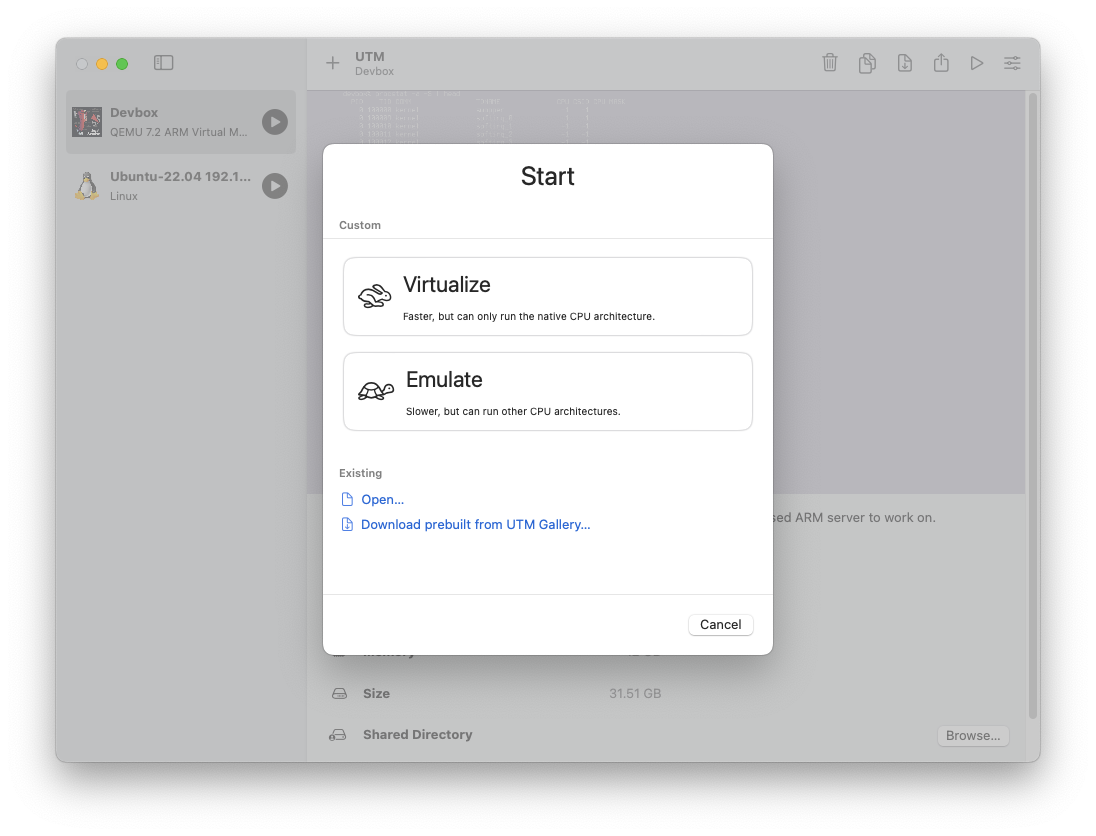
\includegraphics[width=0.6\linewidth]{1}
  \caption{Seclect Virtualize}
  \label{fig:utm-start}
\end{figure}

\begin{figure}
  \centering
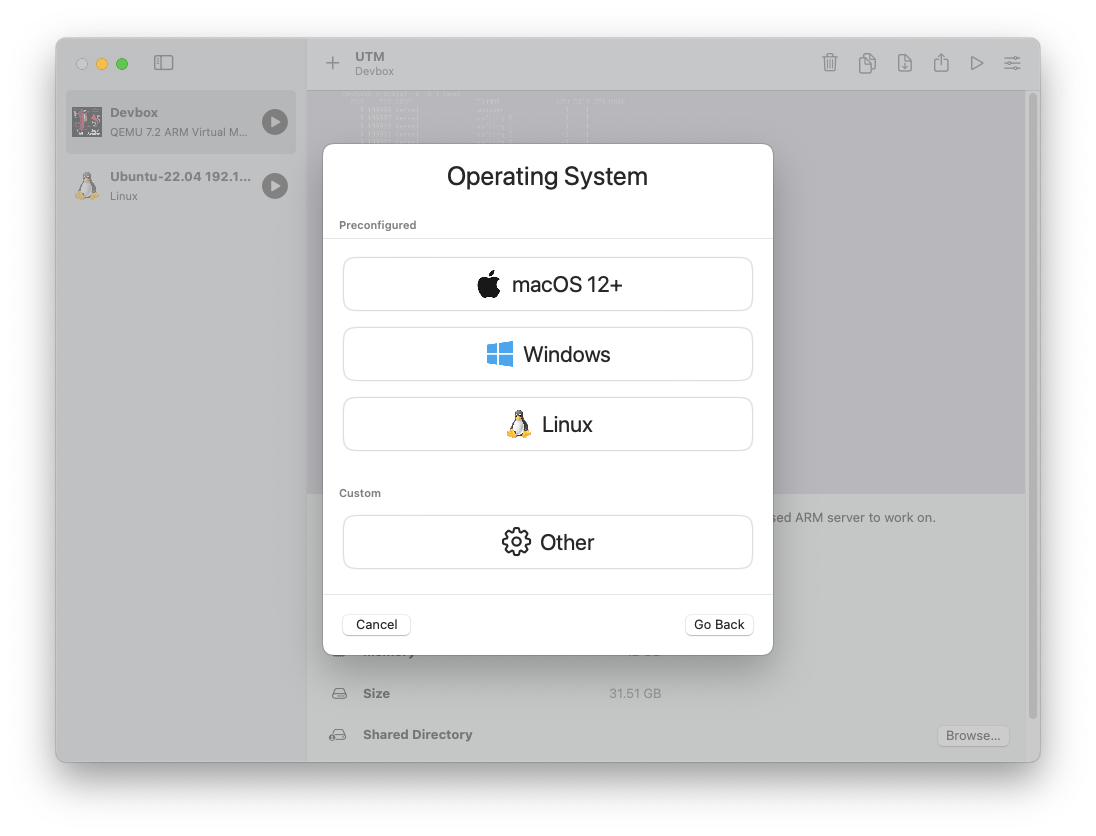
\includegraphics[width=0.6\linewidth]{2}
  \caption{Select Other}
  \label{fig:utm-other}
\end{figure}

\begin{figure}
  \centering
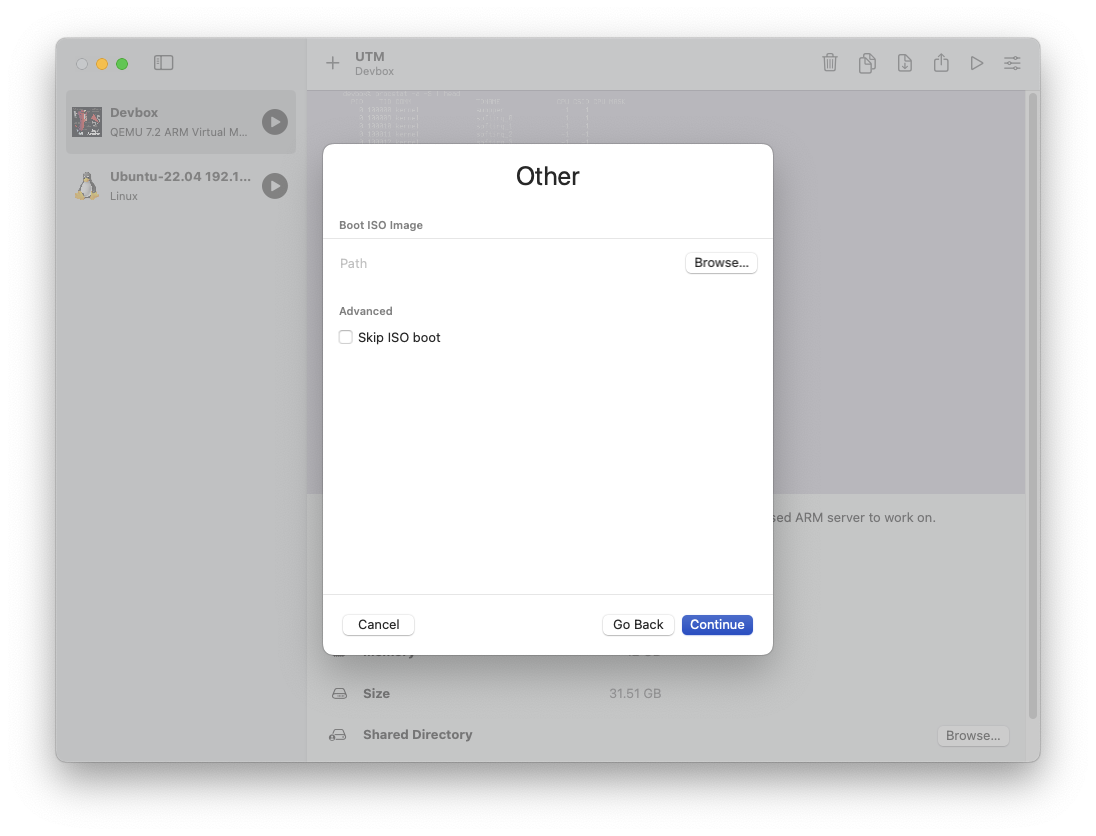
\includegraphics[width=0.6\linewidth]{3}
  \caption{Browe to the ISO}
  \label{fig:utm-browse}
\end{figure}

\begin{figure}
  \centering
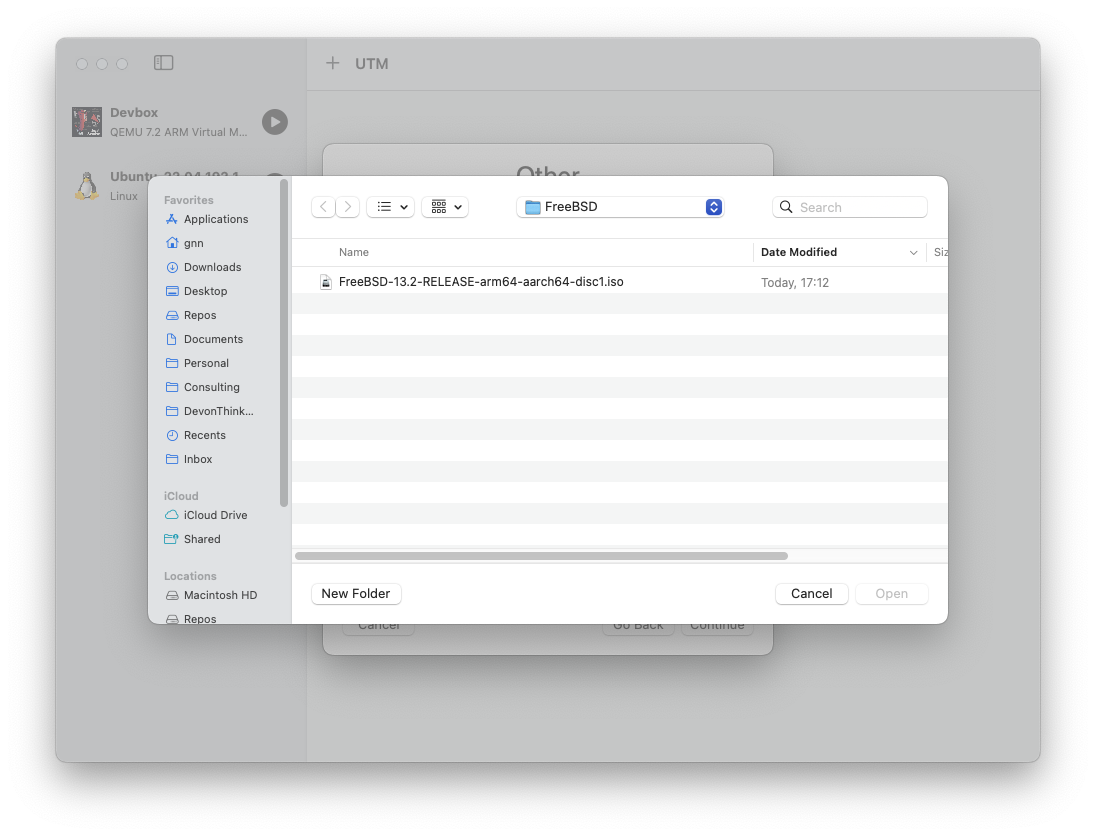
\includegraphics[width=0.6\linewidth]{8}
  \caption{Select the ISO}
  \label{fig:utm-iso}
\end{figure}

\begin{figure}
  \centering
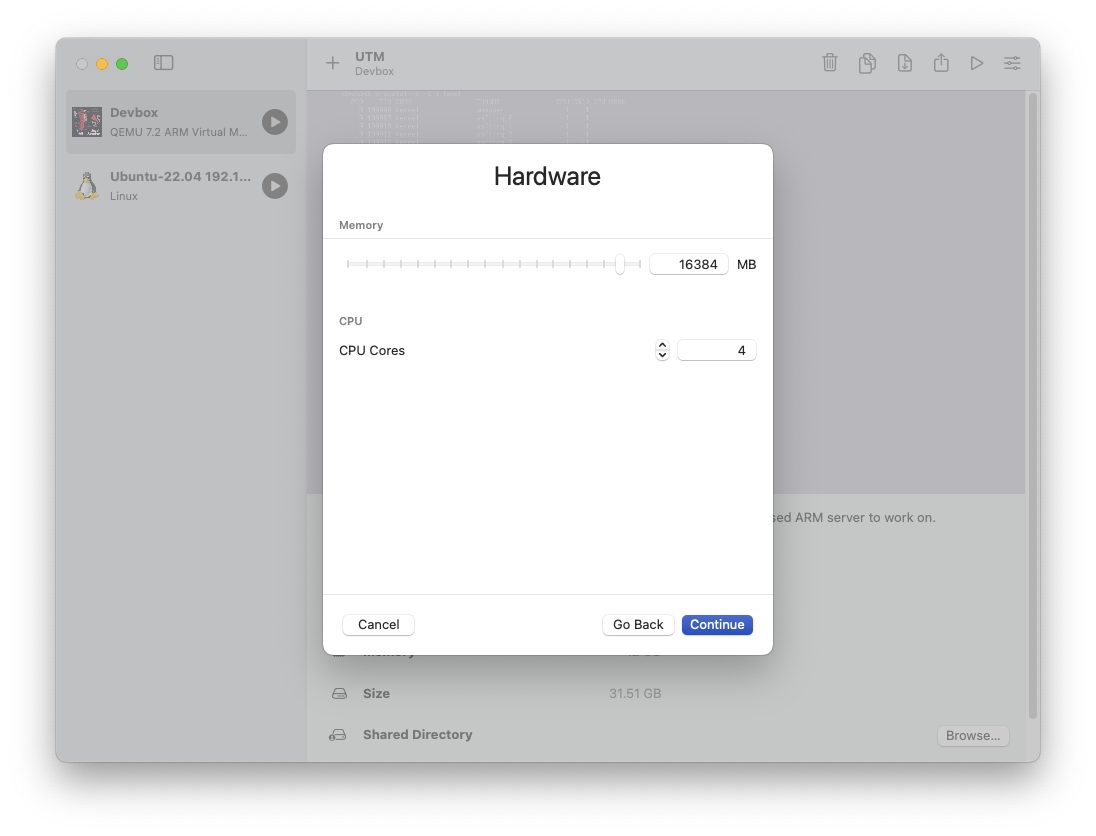
\includegraphics[width=0.6\linewidth]{4}
  \caption{Select 16G of RAM and 4 cores}
  \label{fig:utm-sizing}
\end{figure}

\begin{figure}
  \centering
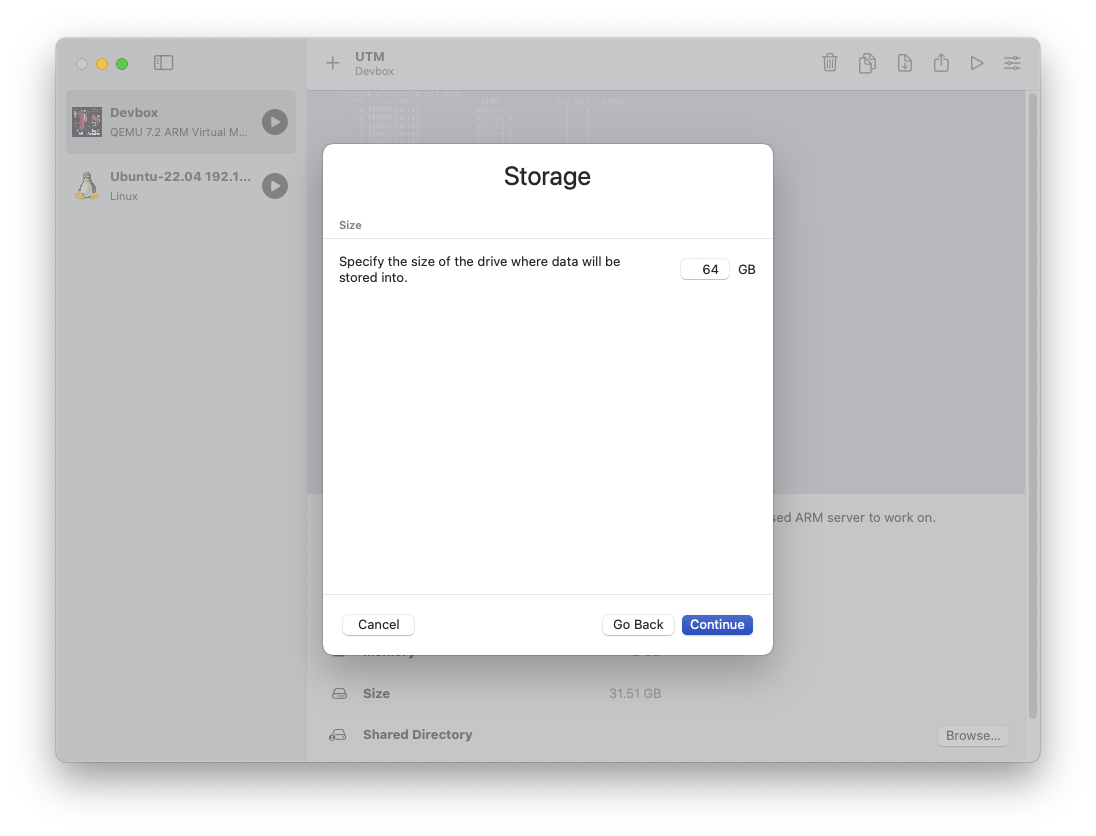
\includegraphics[width=0.6\linewidth]{5}
  \caption{Select the default 64G disk size}
  \label{fig:utm-disk}
\end{figure}

\begin{figure}
  \centering
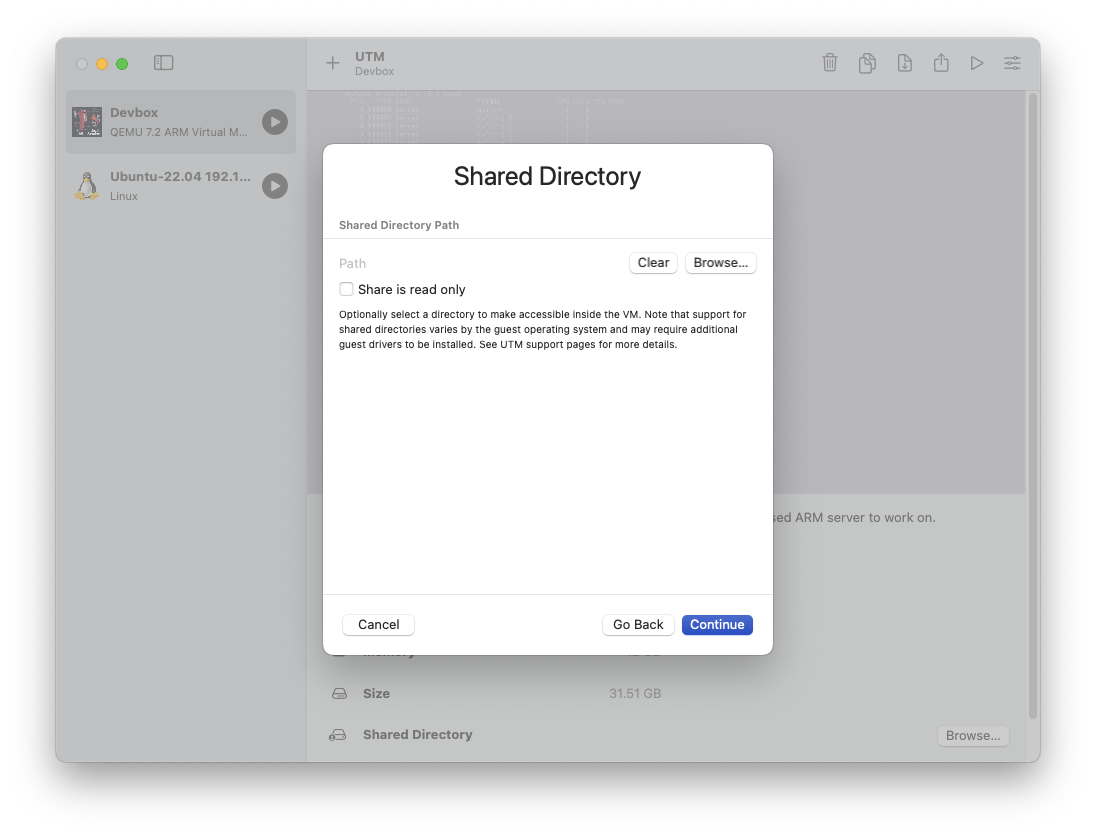
\includegraphics[width=0.6\linewidth]{6}
  \caption{Do not select a Shared Directory}
  \label{fig:utm-shared}
\end{figure}

\begin{figure}
  \centering
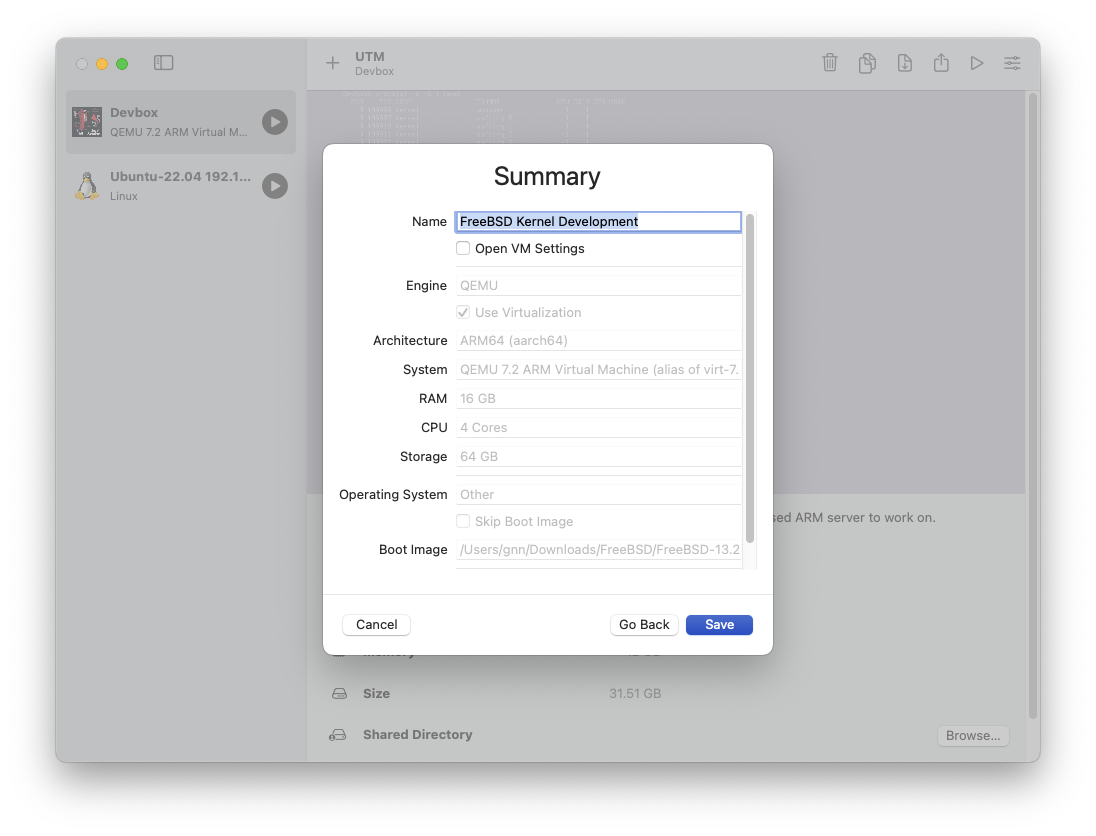
\includegraphics[width=0.6\linewidth]{7}
  \caption{Name your Virtual Machine}
  \label{fig:utm-summary}
\end{figure}

\begin{figure}
  \centering
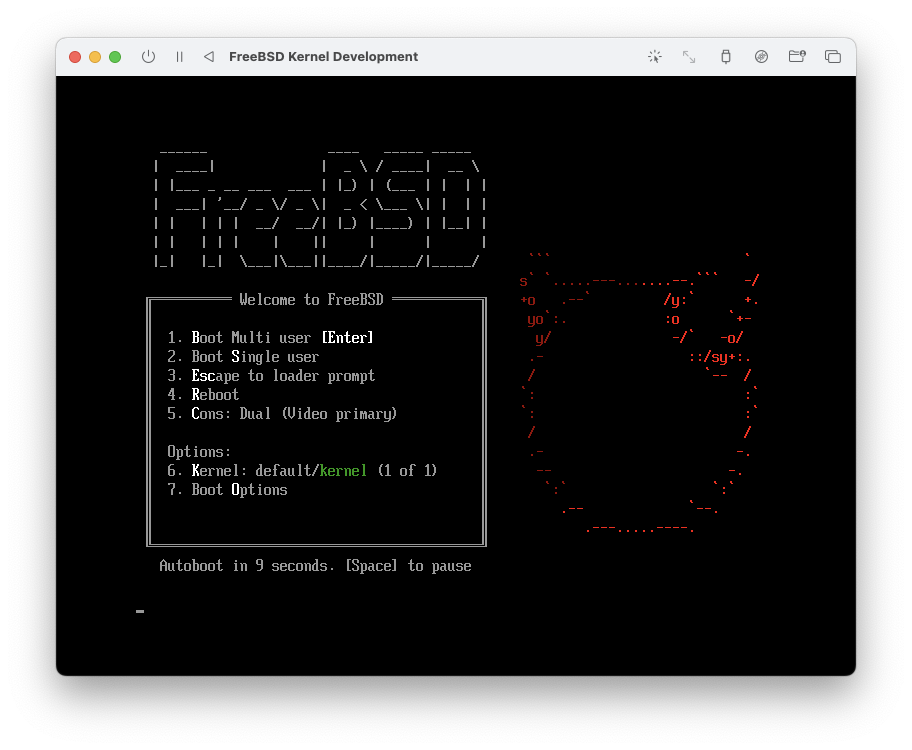
\includegraphics[width=0.6\linewidth]{9}
  \caption{FreeBSD Installer Boot Screen}
  \label{fig:utm-fbsd-install-boot}
\end{figure}

\begin{figure}
  \centering
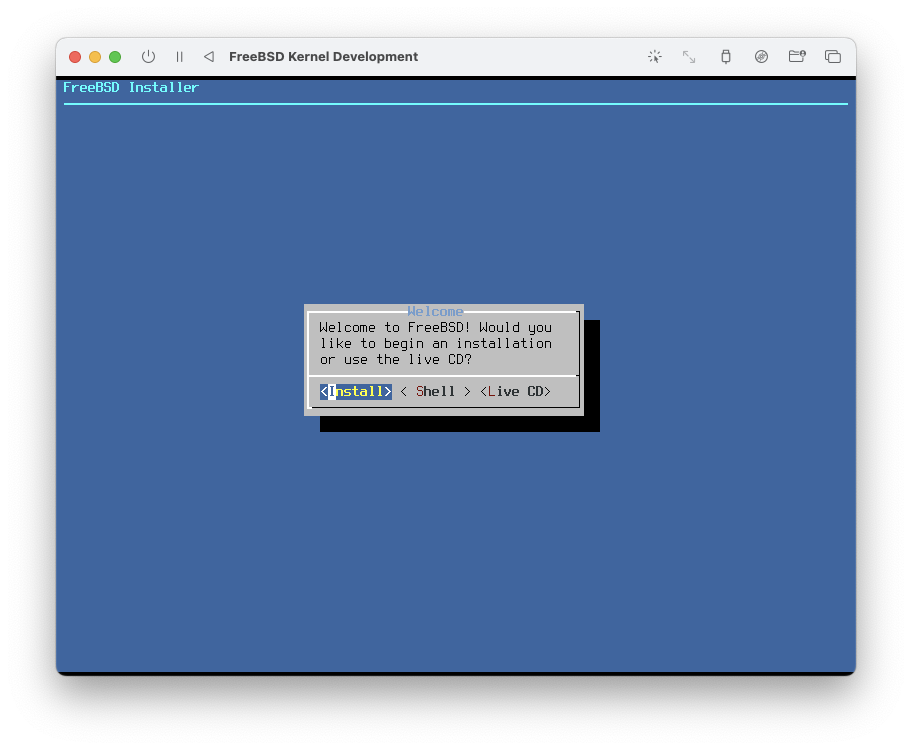
\includegraphics[width=0.6\linewidth]{10}
  \caption{Selec the Install option.}
  \label{fig:utm-fbsd-install}
\end{figure}

\begin{figure}
  \centering
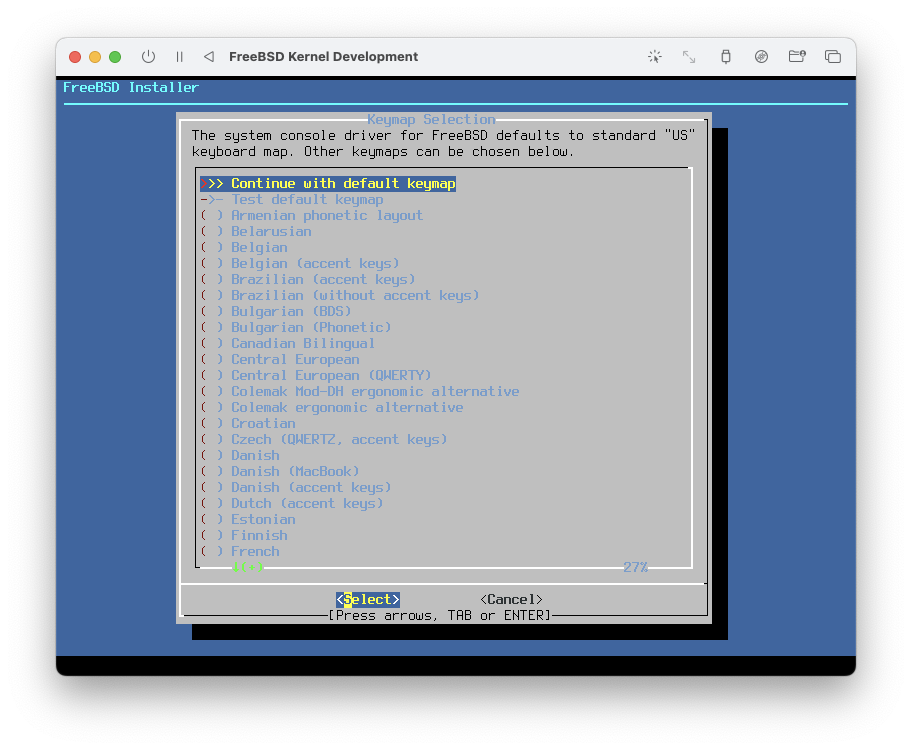
\includegraphics[width=0.6\linewidth]{11}
  \caption{Continued with the default keymap}
  \label{fig:utm-fbsd-keymap}
\end{figure}

\begin{figure}
  \centering
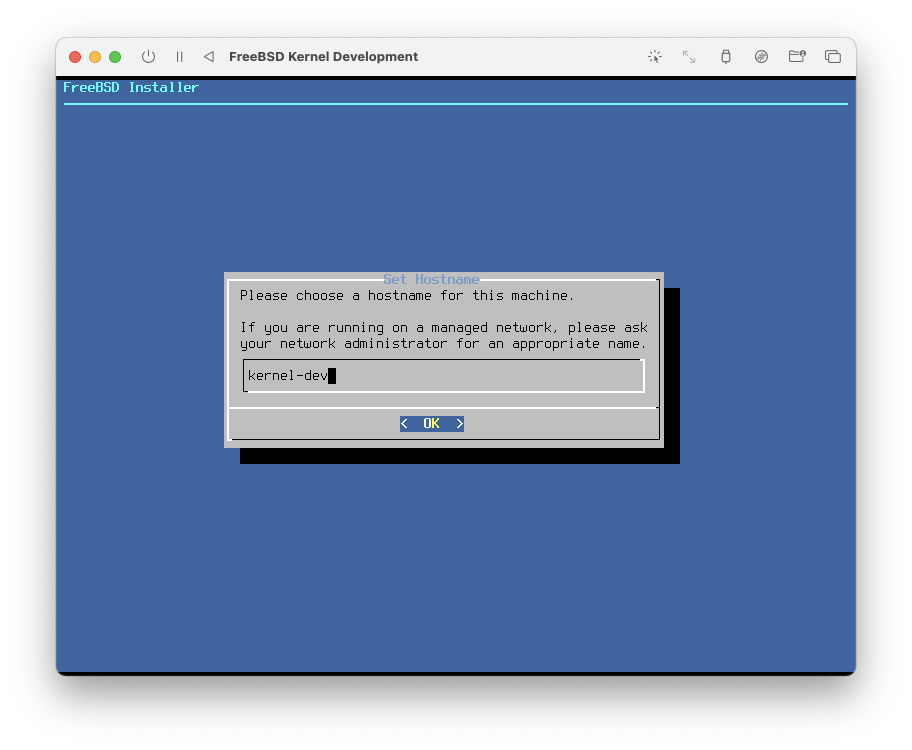
\includegraphics[width=0.6\linewidth]{12}
  \caption{Name your host: kernel-dev}
  \label{fig:utm-fbsd-name}
\end{figure}

\begin{figure}
  \centering
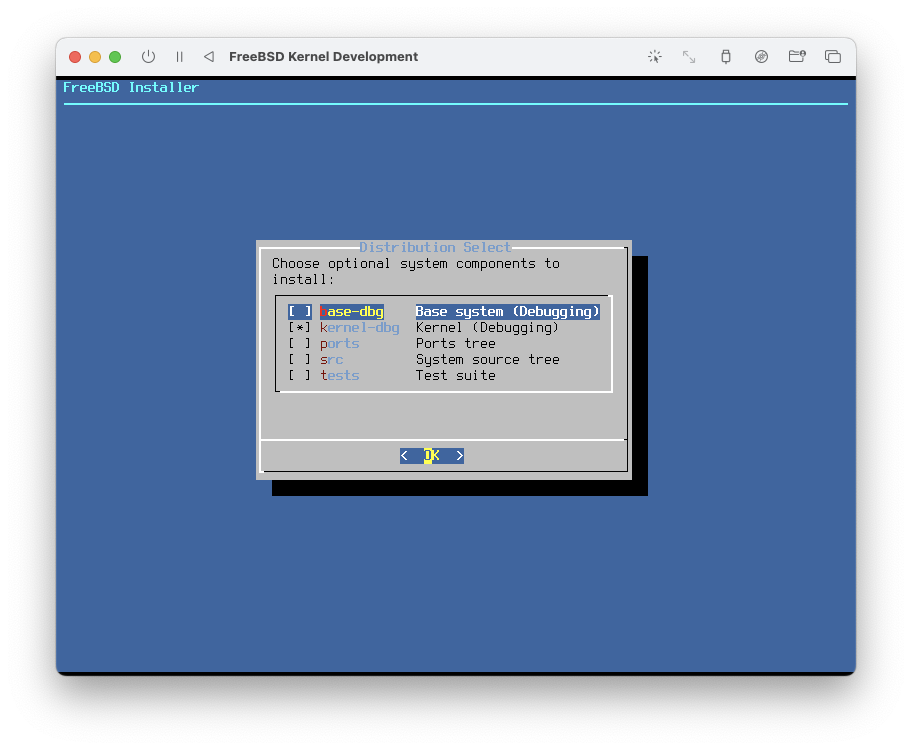
\includegraphics[width=0.6\linewidth]{13}
  \caption{Go with the defaults}
  \label{fig:utm-fbsd-components}
\end{figure}

\begin{figure}
  \centering
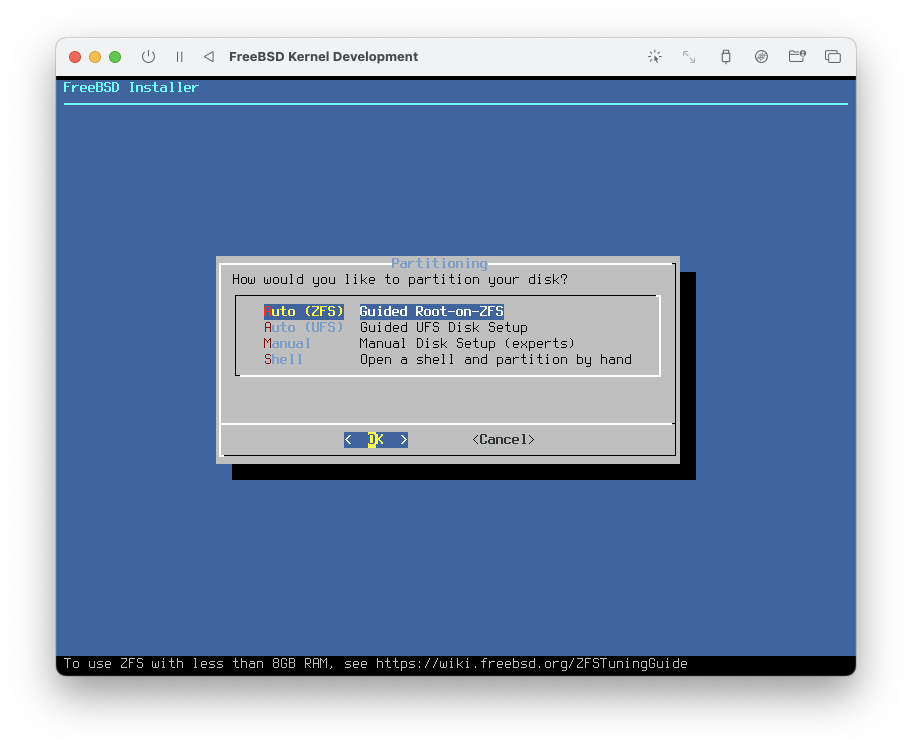
\includegraphics[width=0.6\linewidth]{14}
  \caption{Select ZFS as your filesystem}
  \label{fig:utm-fbsd-zfs}
\end{figure}

\begin{figure}
  \centering
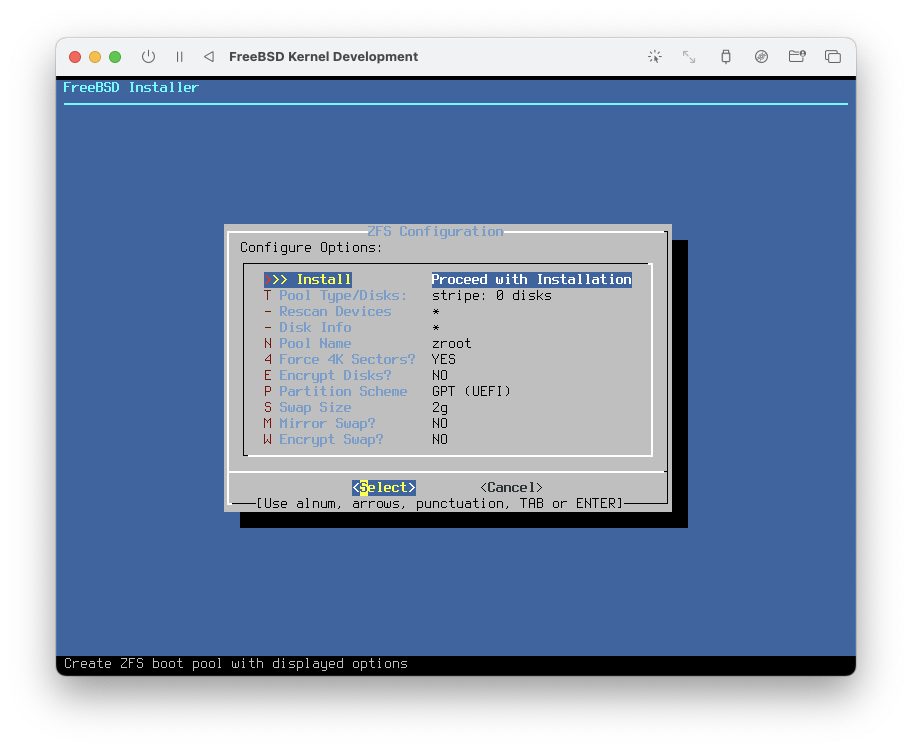
\includegraphics[width=0.6\linewidth]{15}
  \caption{THe ZFS default are sufficient.}
  \label{fig:utm-fbsd-zfs-defaults}
\end{figure}

\begin{figure}
  \centering
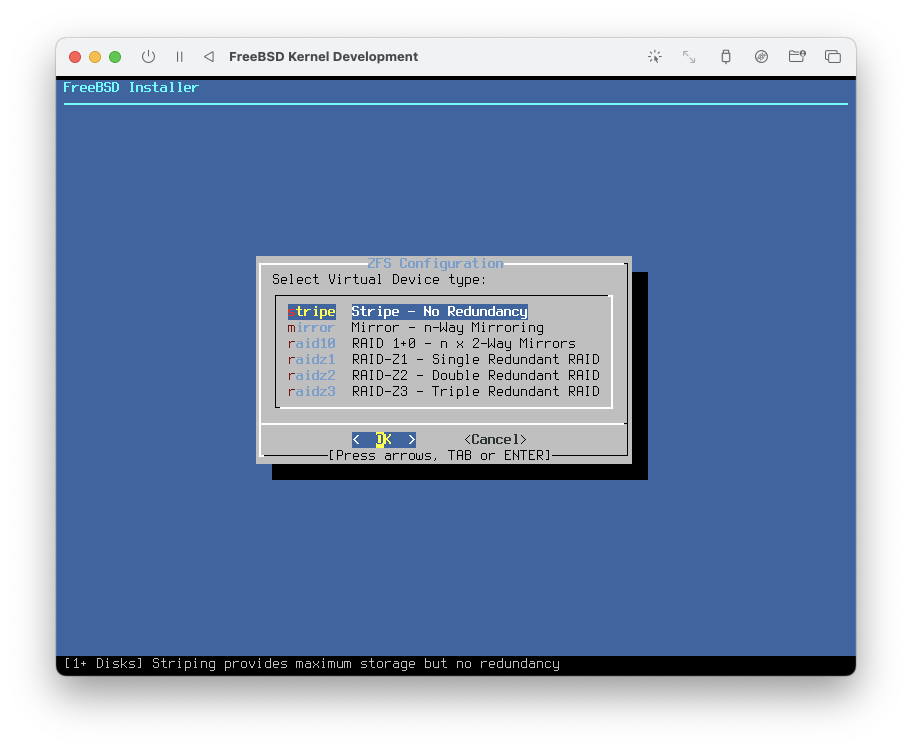
\includegraphics[width=0.6\linewidth]{16}
  \caption{Stripe is all you can do with one disk}
  \label{fig:utm-fbsd-stripe}
\end{figure}

\begin{figure}
  \centering
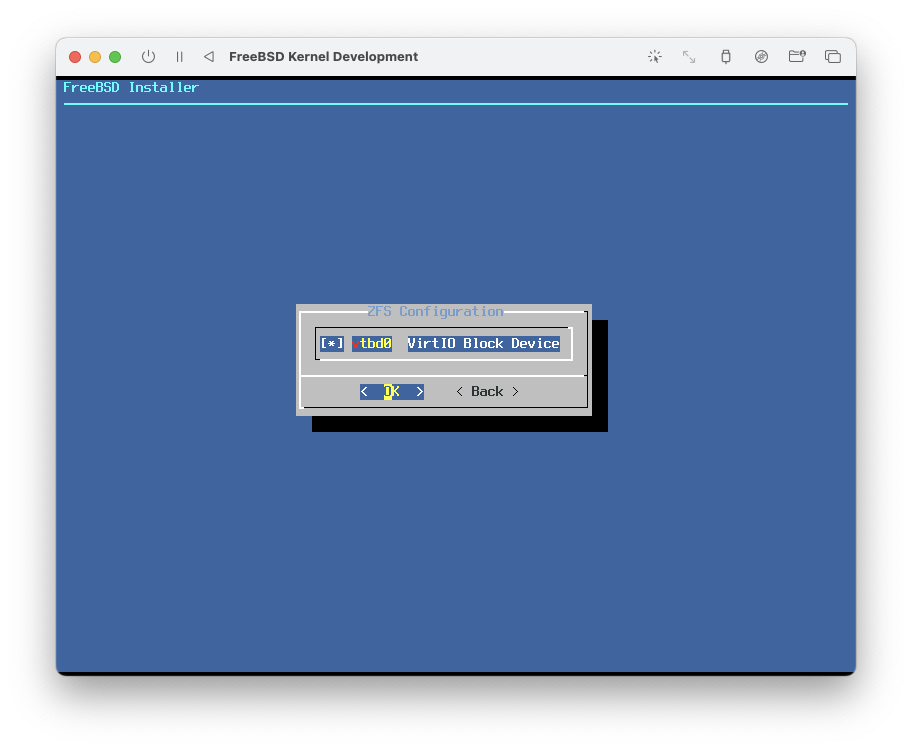
\includegraphics[width=0.6\linewidth]{17}
  \caption{There is only one disk, select it.}
  \label{fig:utm-fbsd-disk}
\end{figure}

\begin{figure}
  \centering
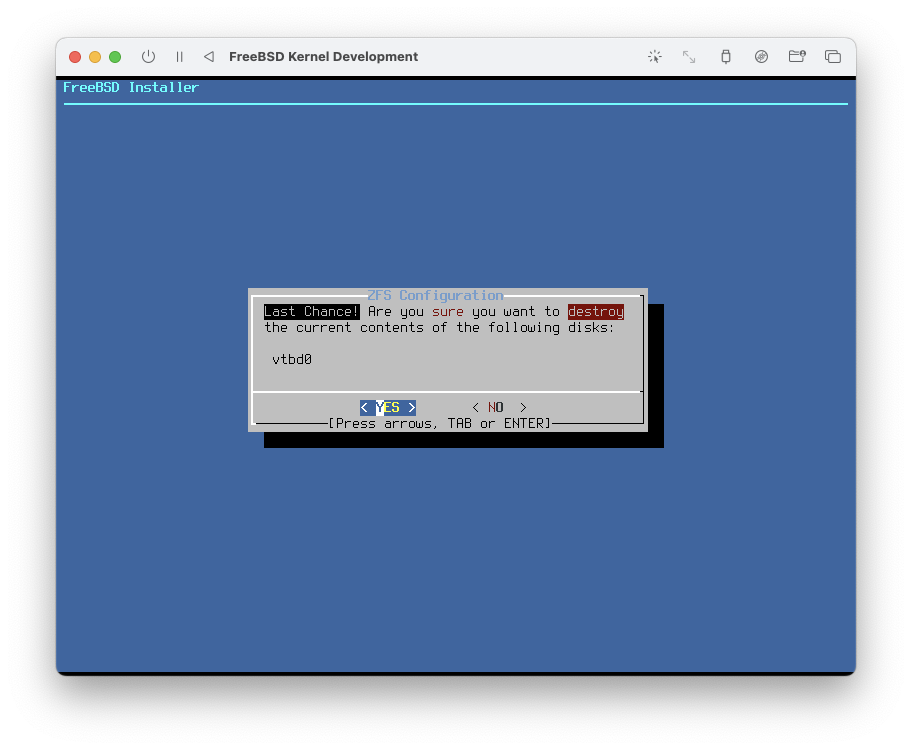
\includegraphics[width=0.6\linewidth]{19}
  \caption{Last chance, select YES.}
  \label{fig:utm-fbsd-last}
\end{figure}

\begin{figure}
  \centering
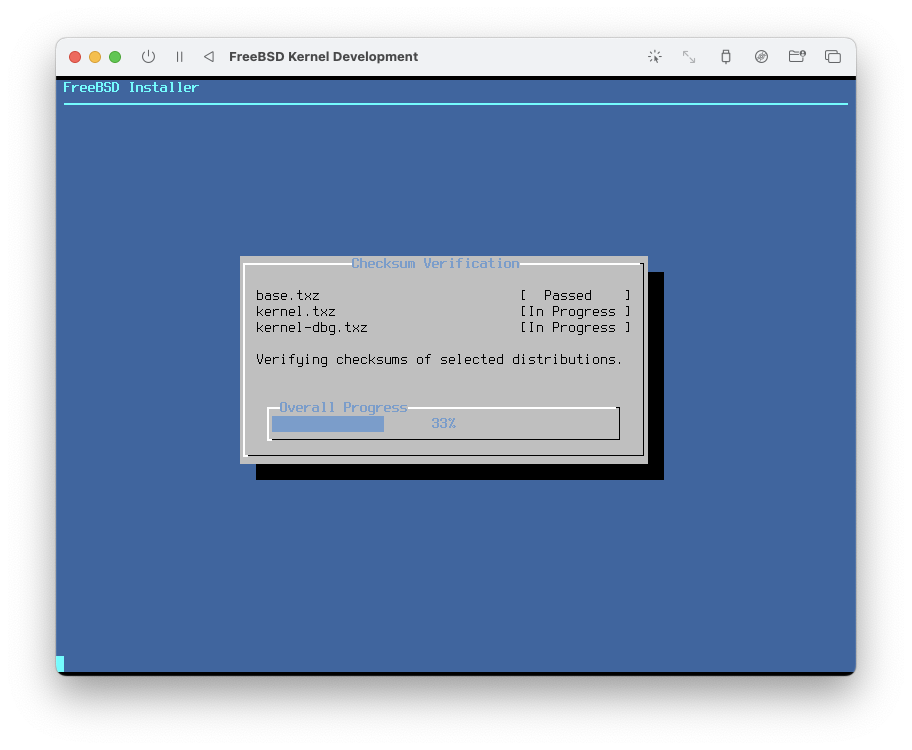
\includegraphics[width=0.6\linewidth]{20}
  \caption{Installing}
  \label{fig:utm-fbsd-installing}
\end{figure}

\begin{figure}
  \centering
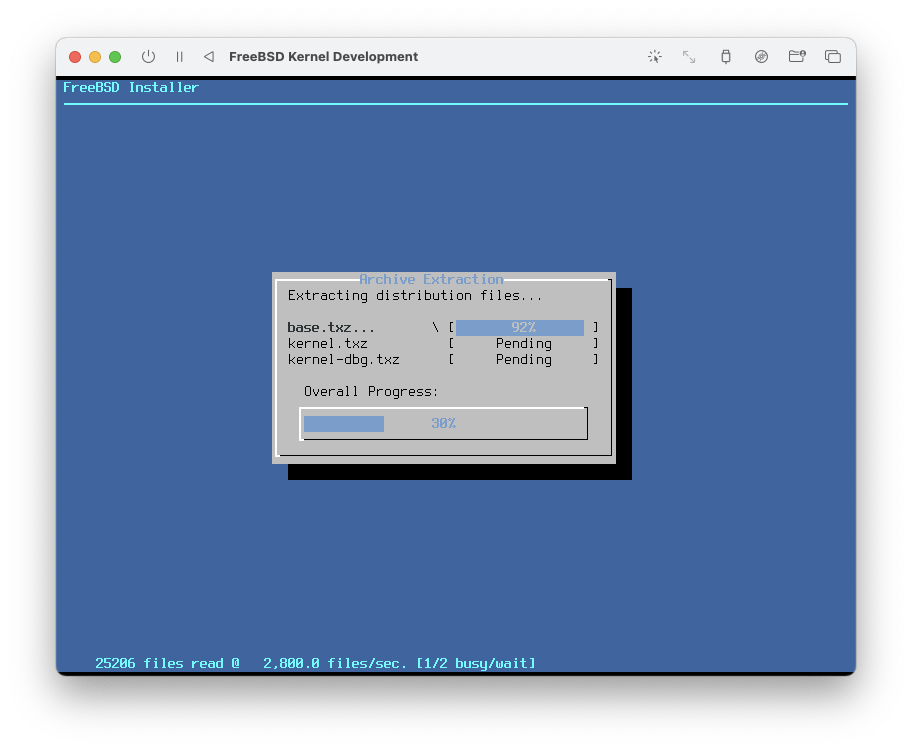
\includegraphics[width=0.6\linewidth]{21}
  \caption{Extracting files}
  \label{fig:utm-fbsd-extractin}
\end{figure}

\begin{figure}
  \centering
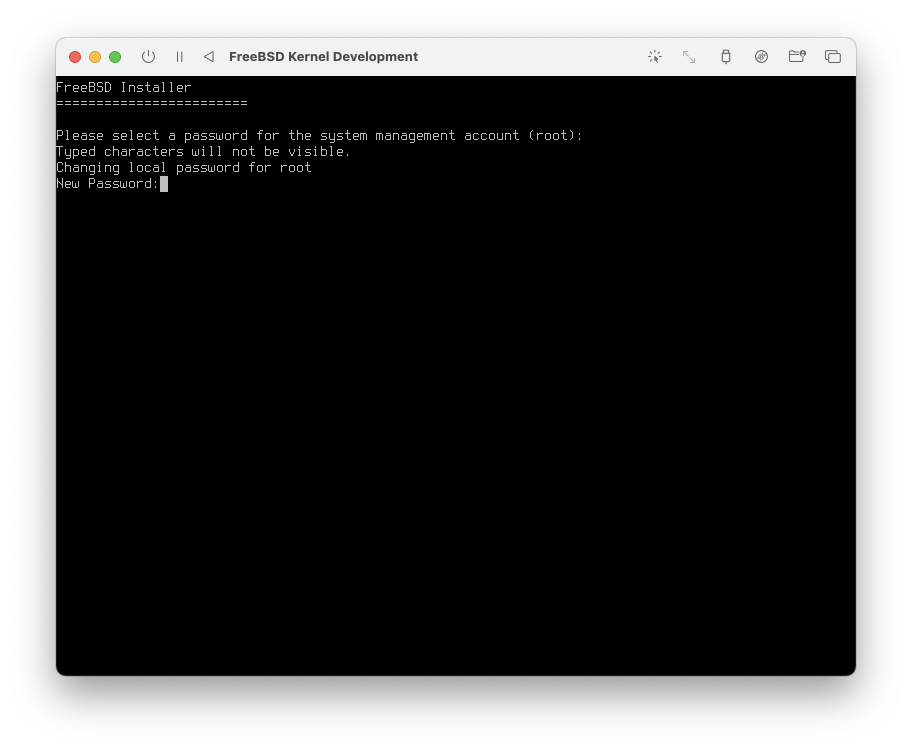
\includegraphics[width=0.6\linewidth]{22}
  \caption{Select a root password}
  \label{fig:utm-fbsd-rootpw}
\end{figure}

\begin{figure}
  \centering
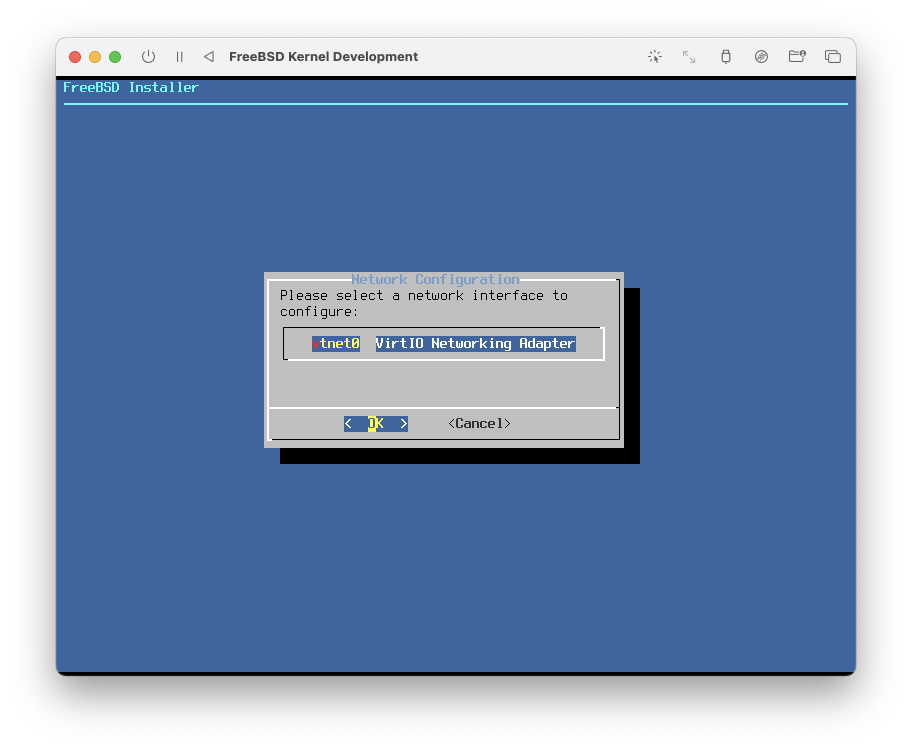
\includegraphics[width=0.6\linewidth]{23}
  \caption{There is only one network device}
  \label{fig:utm-fbsd-netdev}
\end{figure}

\begin{figure}
  \centering
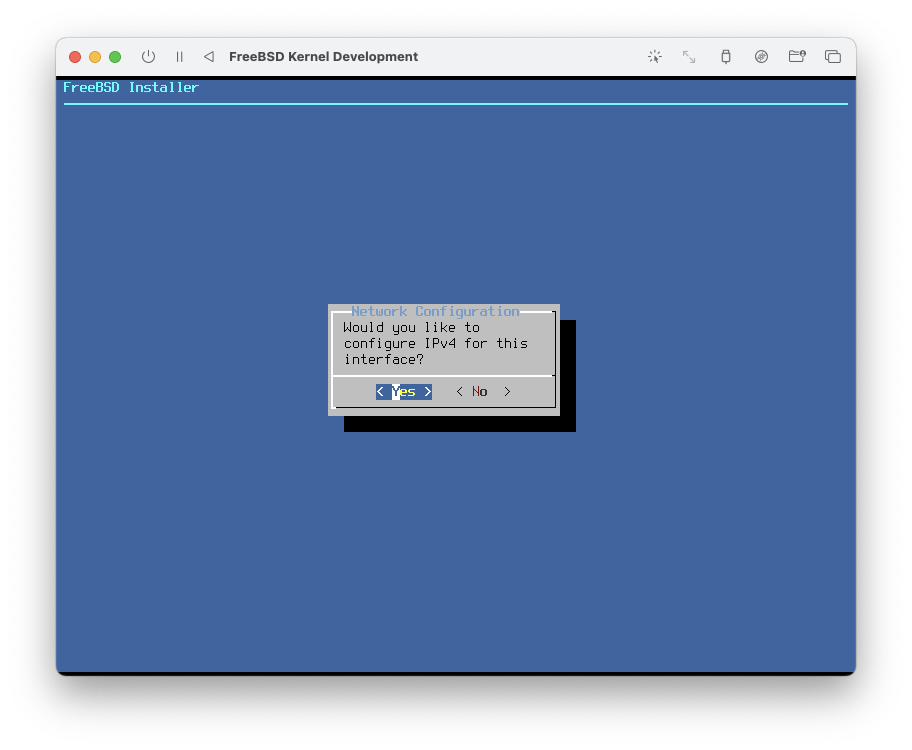
\includegraphics[width=0.6\linewidth]{24}
  \caption{Use IPv4}
  \label{fig:utm-fbsd-ipv4}
\end{figure}

\begin{figure}
  \centering
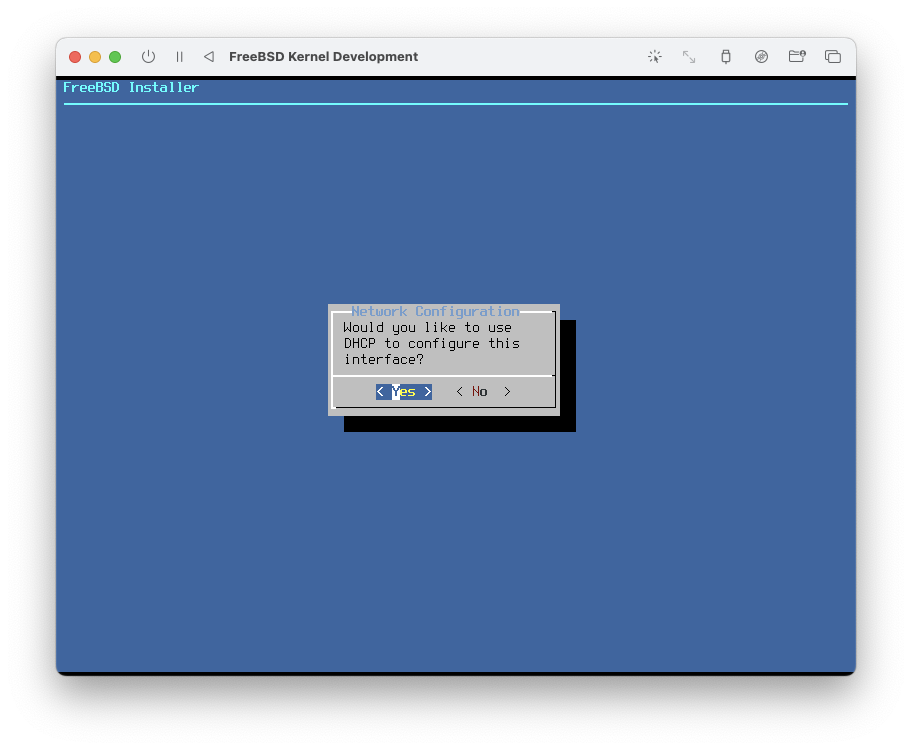
\includegraphics[width=0.6\linewidth]{25}
  \caption{Use DHCP for IPv4}
  \label{fig:utm-fbsd-dhcp}
\end{figure}

\begin{figure}
  \centering
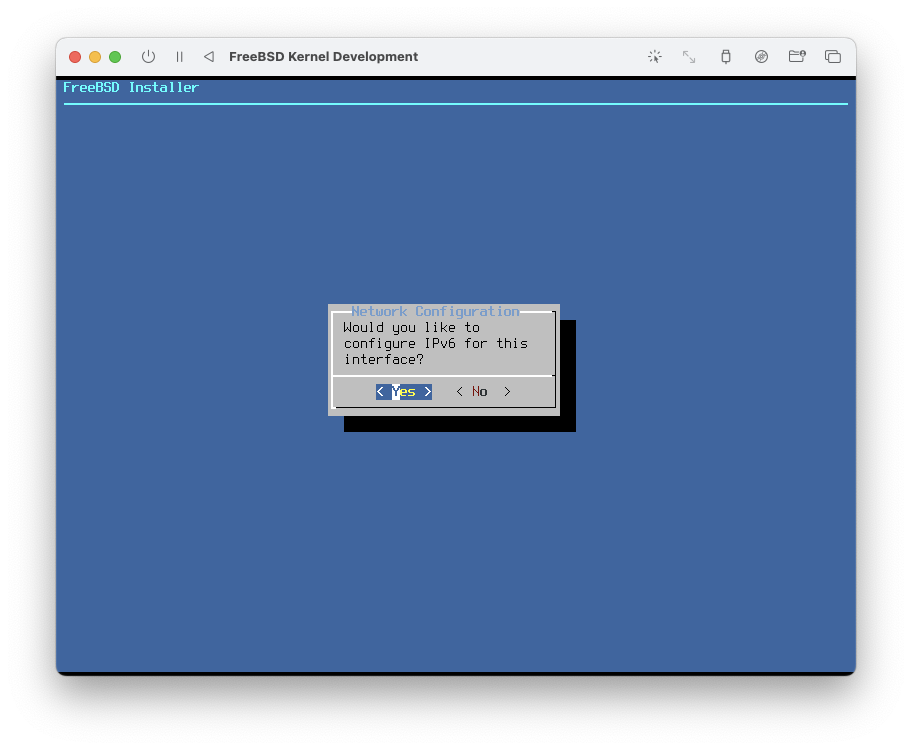
\includegraphics[width=0.6\linewidth]{26}
  \caption{Do not configure IPv6}
  \label{fig:utm-fbsd-ipv6}
\end{figure}

\begin{figure}
  \centering
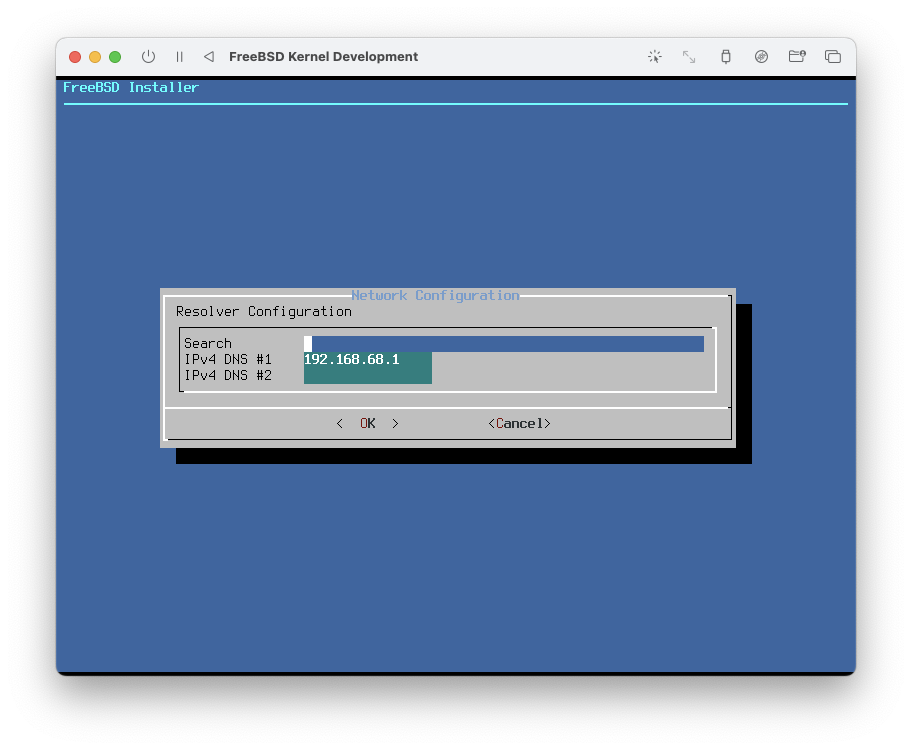
\includegraphics[width=0.6\linewidth]{27}
  \caption{Accept the default DNS resolver settings}
  \label{fig:utm-fbsd-dns}
\end{figure}

\begin{figure}
  \centering
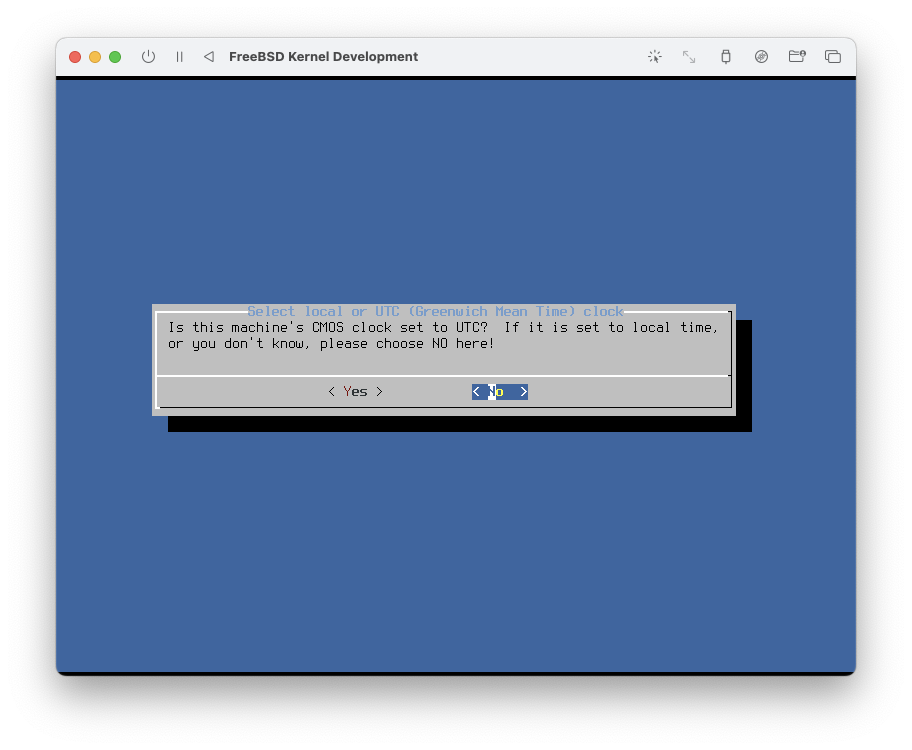
\includegraphics[width=0.6\linewidth]{28}
  \caption{Start setting the clock, select NO}
  \label{fig:utm-fbsd-cmos}
\end{figure}

\begin{figure}
  \centering
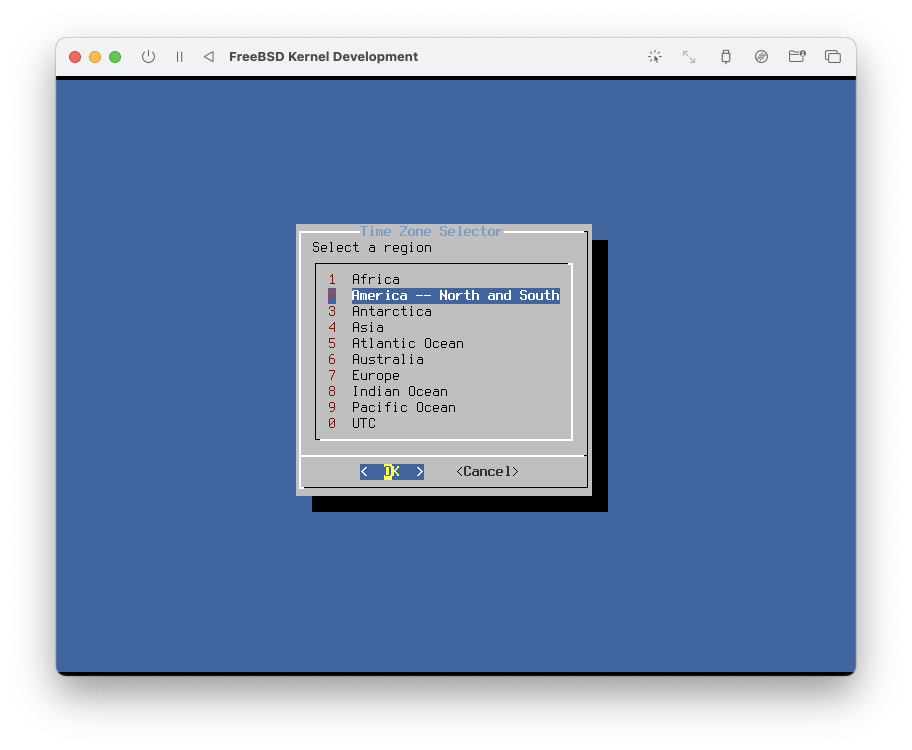
\includegraphics[width=0.6\linewidth]{29}
  \caption{We're setting this up in America}
  \label{fig:utm-fbsd-america}
\end{figure}

\begin{figure}
  \centering
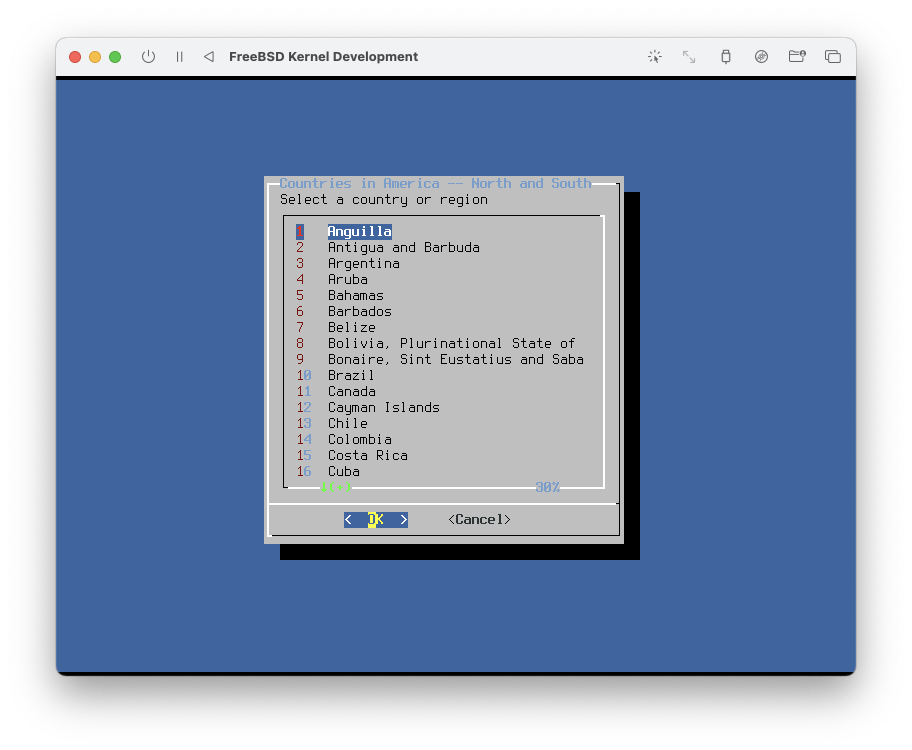
\includegraphics[width=0.6\linewidth]{30}
  \caption{Scroll down to the correct country}
  \label{fig:utm-fbsd-anguilla}
\end{figure}

\begin{figure}
  \centering
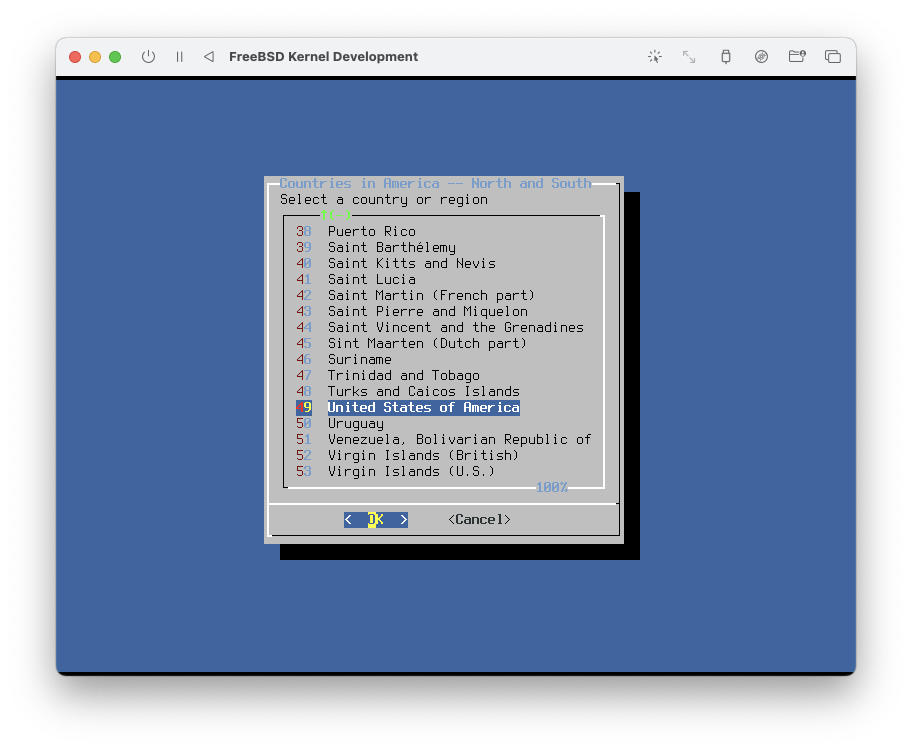
\includegraphics[width=0.6\linewidth]{31}
  \caption{Select United States of America}
  \label{fig:utm-fbsd-usa}
\end{figure}

\begin{figure}
  \centering
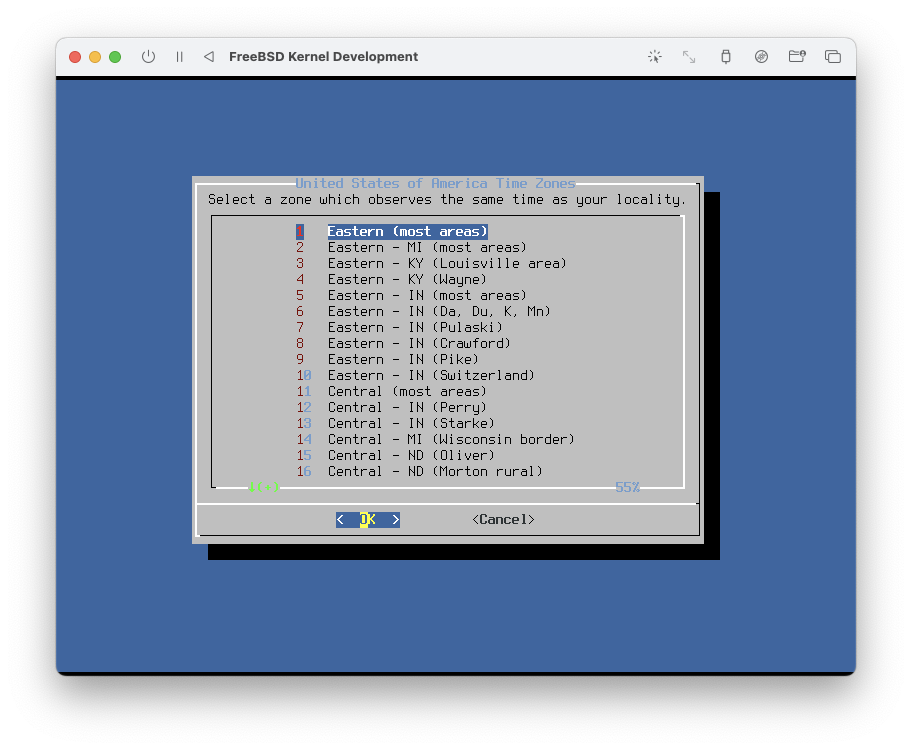
\includegraphics[width=0.6\linewidth]{32}
  \caption{We are in the Eastern timezone}
  \label{fig:utm-fbsd-eastern}
\end{figure}

\begin{figure}
  \centering
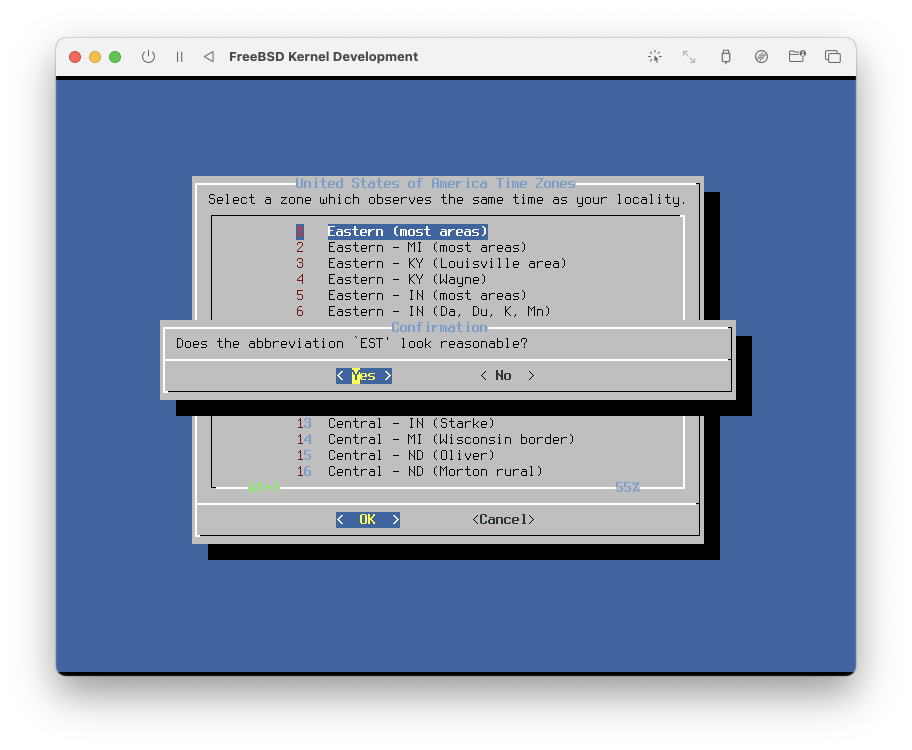
\includegraphics[width=0.6\linewidth]{33}
  \caption{Accept EST}
  \label{fig:utm-fbsd-est}
\end{figure}

\begin{figure}
  \centering
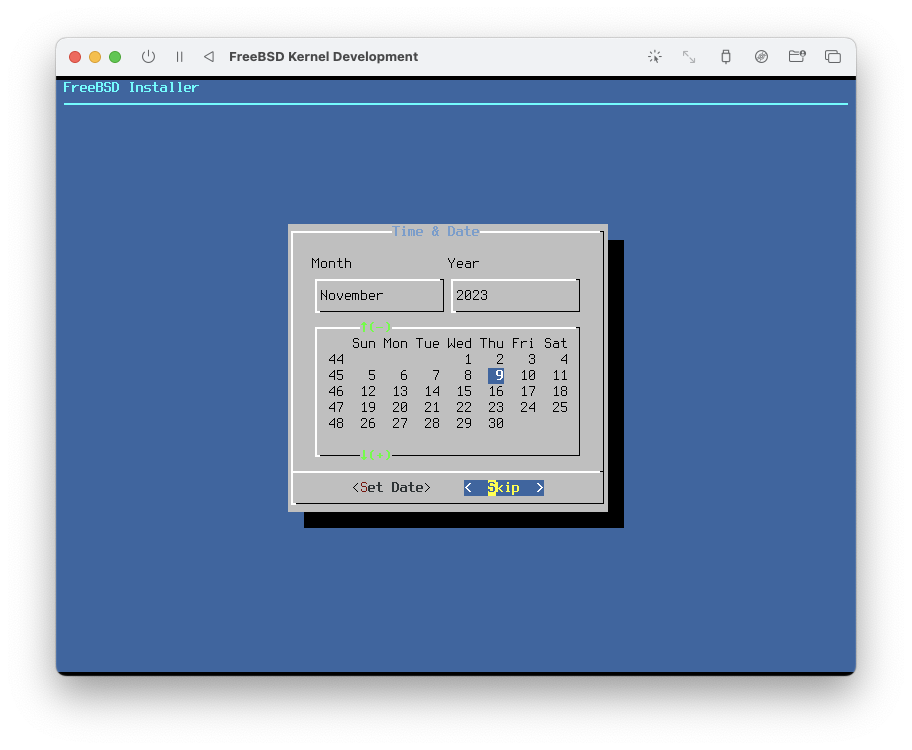
\includegraphics[width=0.6\linewidth]{34}
  \caption{Skip setting the date (ntp will handle this on first boot)}
  \label{fig:utm-fbsd-date}
\end{figure}

\begin{figure}
  \centering
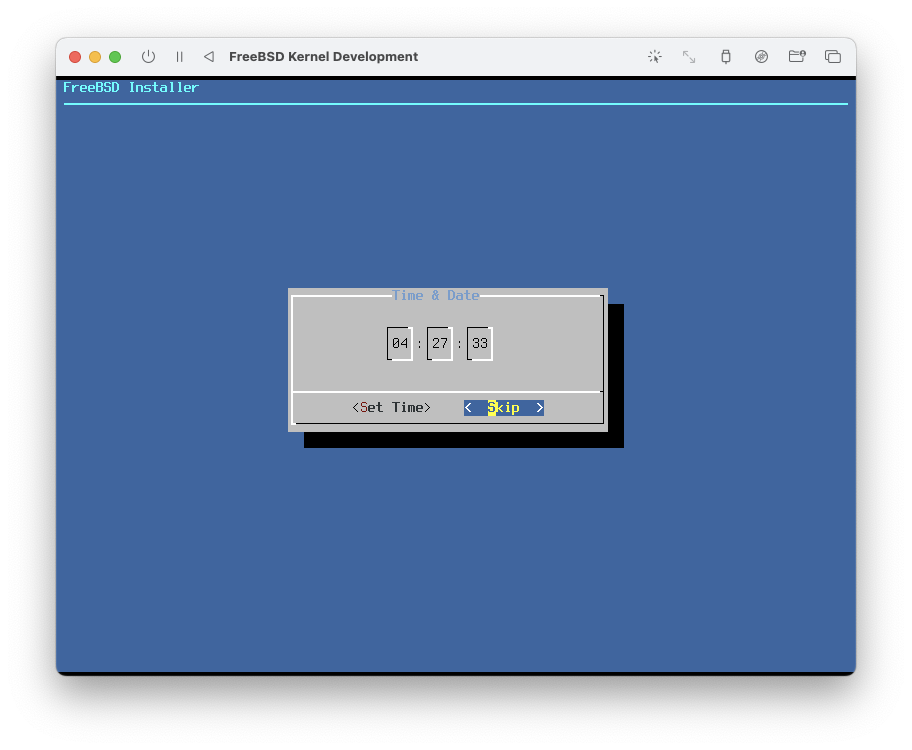
\includegraphics[width=0.6\linewidth]{35}
  \caption{Skip setting the time (ntp will handle this on first boot)}
  \label{fig:utm-fbsd-time}
\end{figure}

\begin{figure}
  \centering
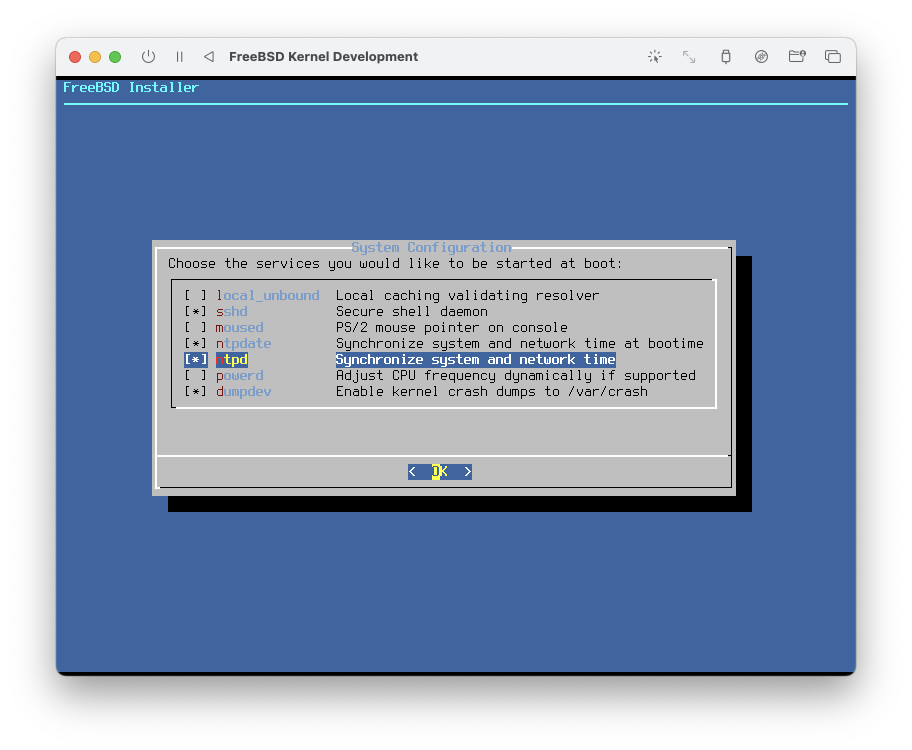
\includegraphics[width=0.6\linewidth]{36}
  \caption{Select both ntpdate and ntpd}
  \label{fig:utm-fbsd-ntp}
\end{figure}

\begin{figure}
  \centering
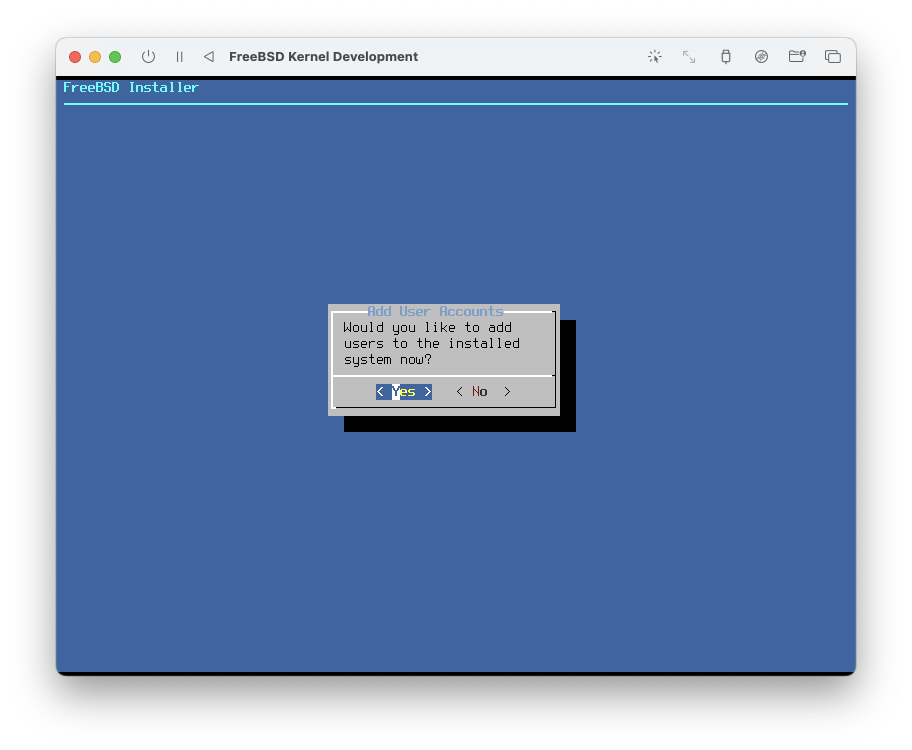
\includegraphics[width=0.6\linewidth]{37}
  \caption{Add a user}
  \label{fig:utm-fbsd-adduser}
\end{figure}

\begin{figure}
  \centering
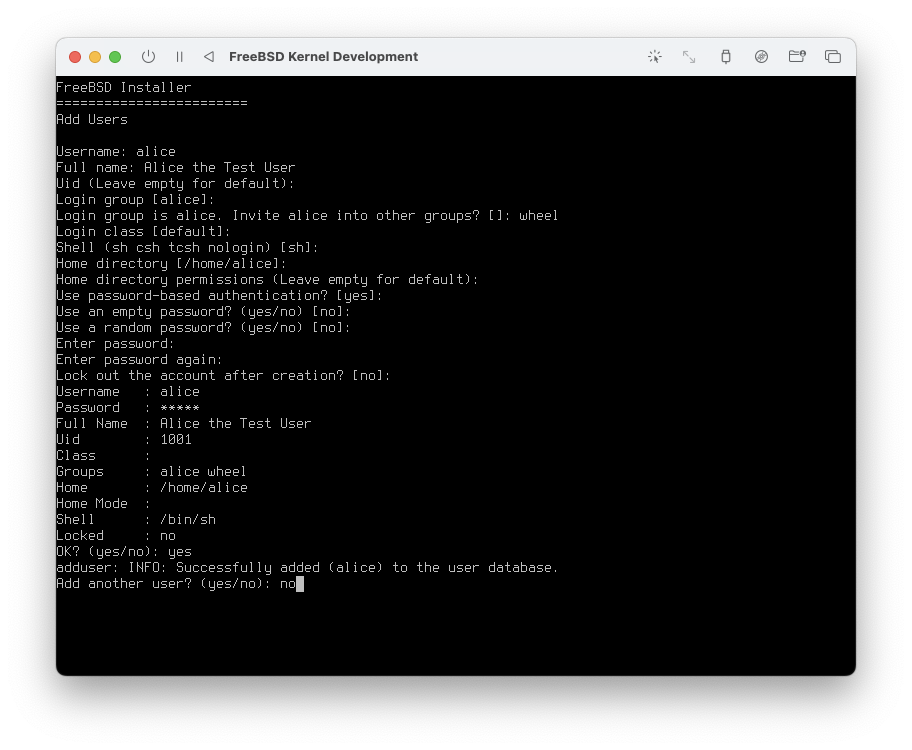
\includegraphics[width=0.6\linewidth]{38}
  \caption{Add a user, example is Alice, use your own login}
  \label{fig:utm-fbsd-alice}
\end{figure}

\begin{figure}
  \centering
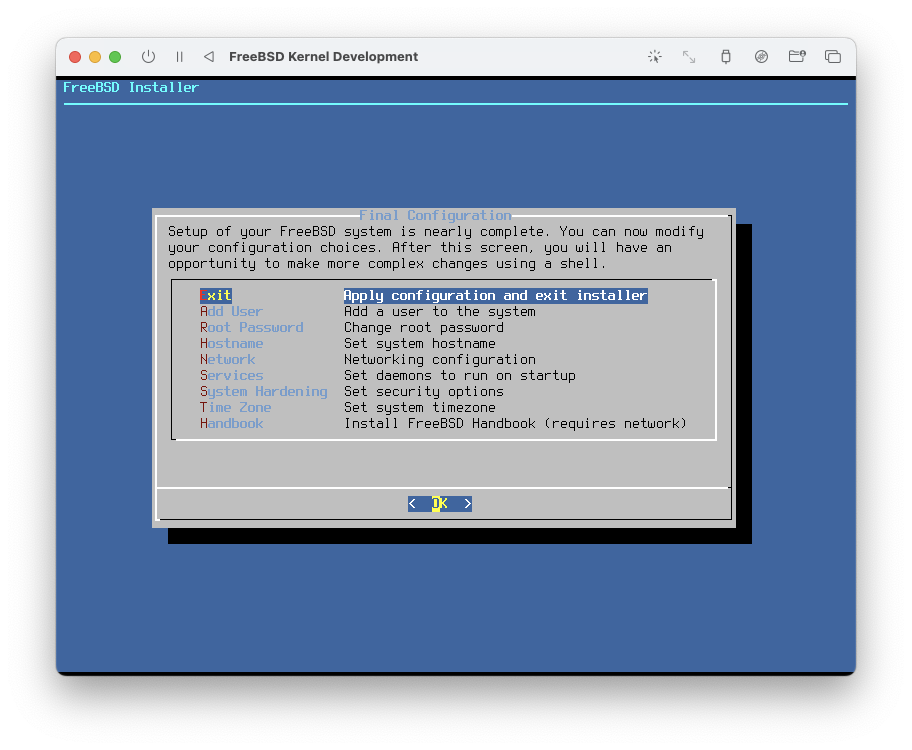
\includegraphics[width=0.6\linewidth]{39}
  \caption{Nearly done, we can Exit}
  \label{fig:utm-fbsd-exit}
\end{figure}

\begin{figure}
  \centering
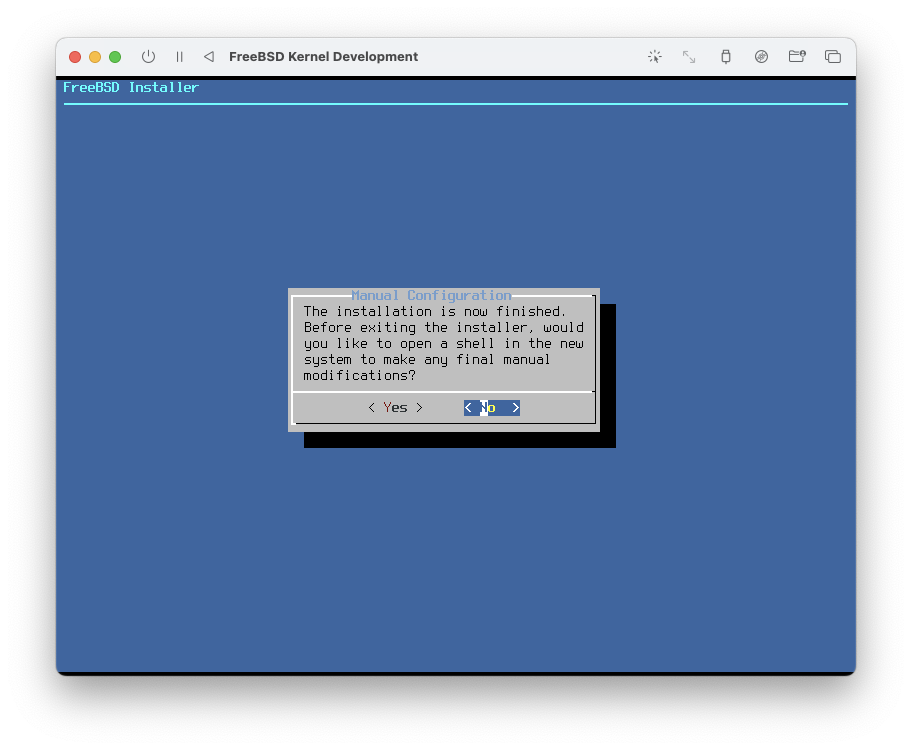
\includegraphics[width=0.6\linewidth]{40}
  \caption{No need for manual modifications, select NO}
  \label{fig:utm-fbsd-nomods}
\end{figure}

\begin{figure}
  \centering
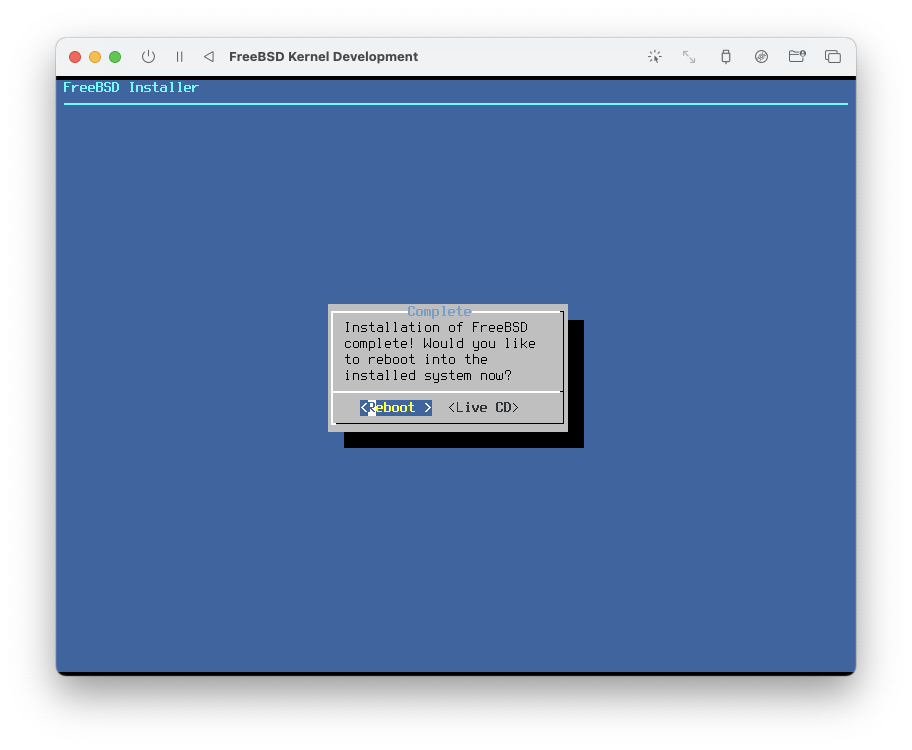
\includegraphics[width=0.6\linewidth]{41}
  \caption{Reboot the system}
  \label{fig:utm-fbsd-reboot}
\end{figure}

Once the system has rebooted, disconnect the CD/DVD ROM ISO from the
Virtual Machine, otherwise the install process will start again.  If
you wind up at the installer prompt a second time, disconnect the
CD/DVD ROM and then reboot the virtual machine again.

\begin{figure}
  \centering
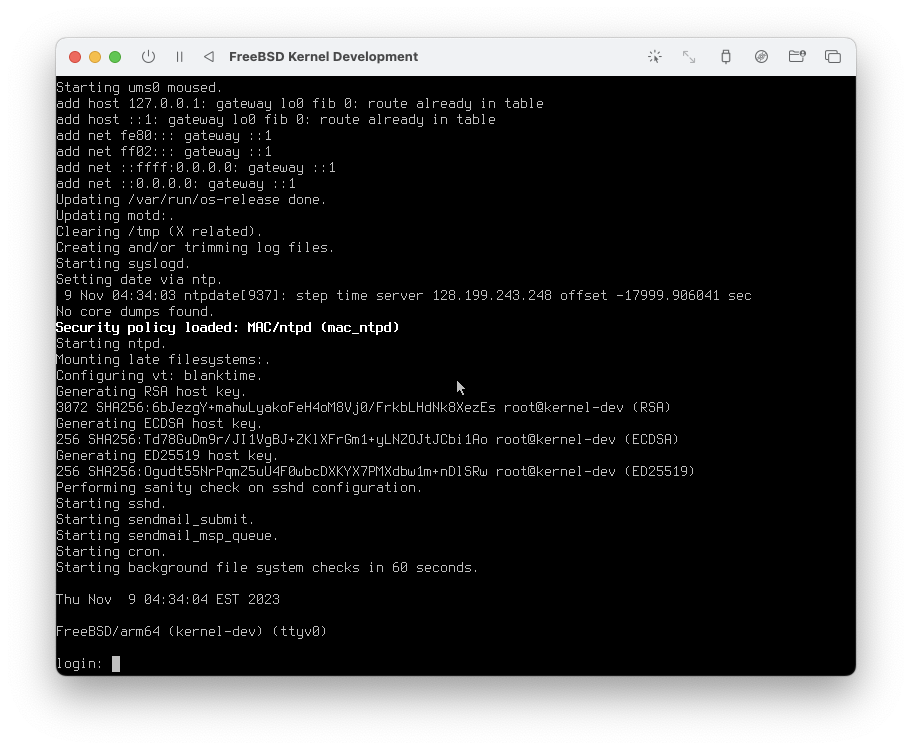
\includegraphics[width=0.6\linewidth]{42}
  \caption{Normal boot to the login prompt.}
  \label{fig:utm-fbsd-login}
\end{figure}

\begin{figure}
  \centering
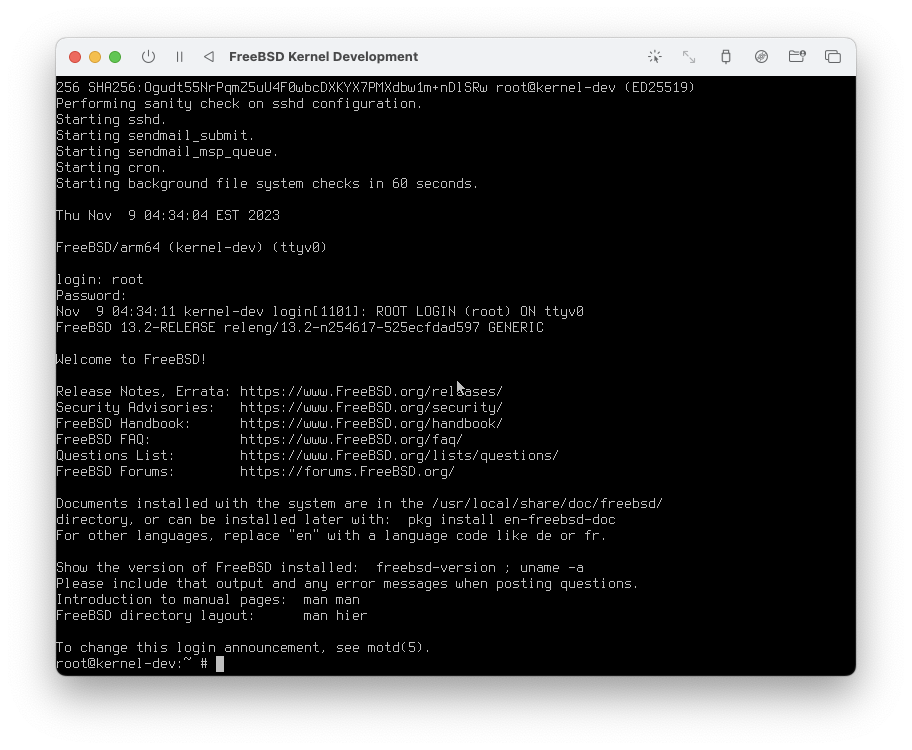
\includegraphics[width=0.6\linewidth]{43}
  \caption{Login to the system as the root user}
  \label{fig:utm-fbsd-root}
\end{figure}

\begin{figure}
  \centering
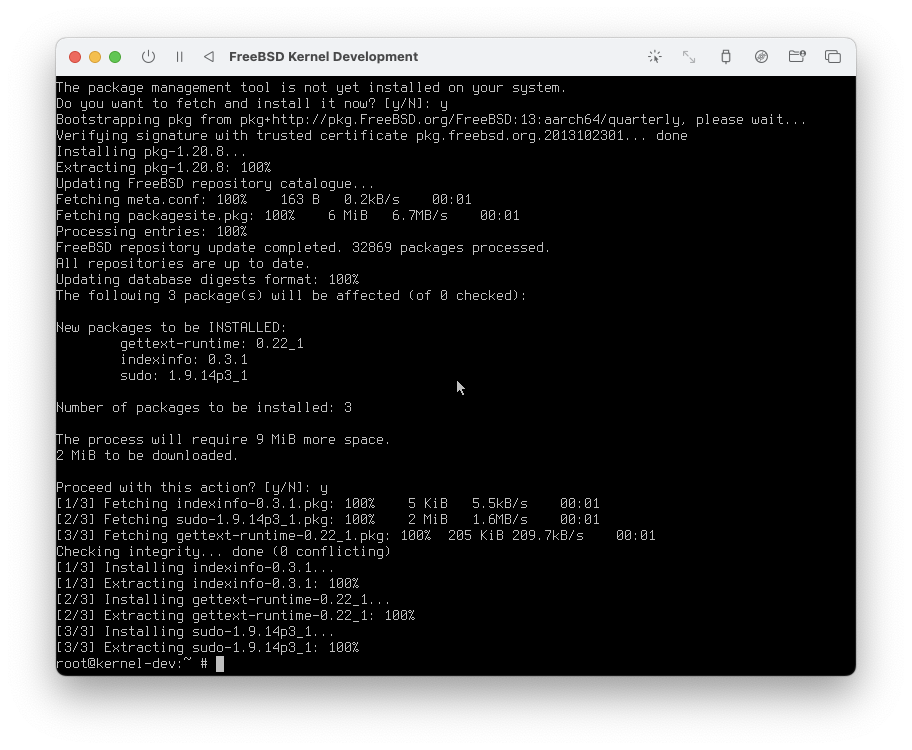
\includegraphics[width=0.6\linewidth]{44}
  \caption{Use the pkg command to install sudo}
  \label{fig:utm-fbsd-pkg}
\end{figure}

\begin{figure}
  \centering
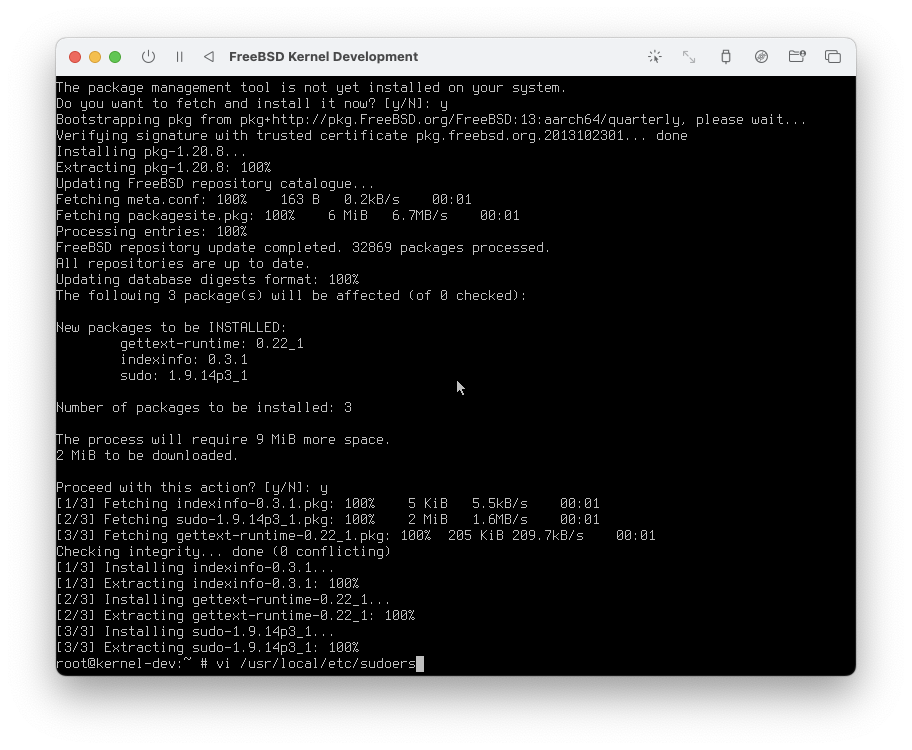
\includegraphics[width=0.6\linewidth]{45}
  \caption{Edit the sudoers file with vi}
  \label{fig:utm-fbsd-sudoers}
\end{figure}

\begin{figure}
  \centering
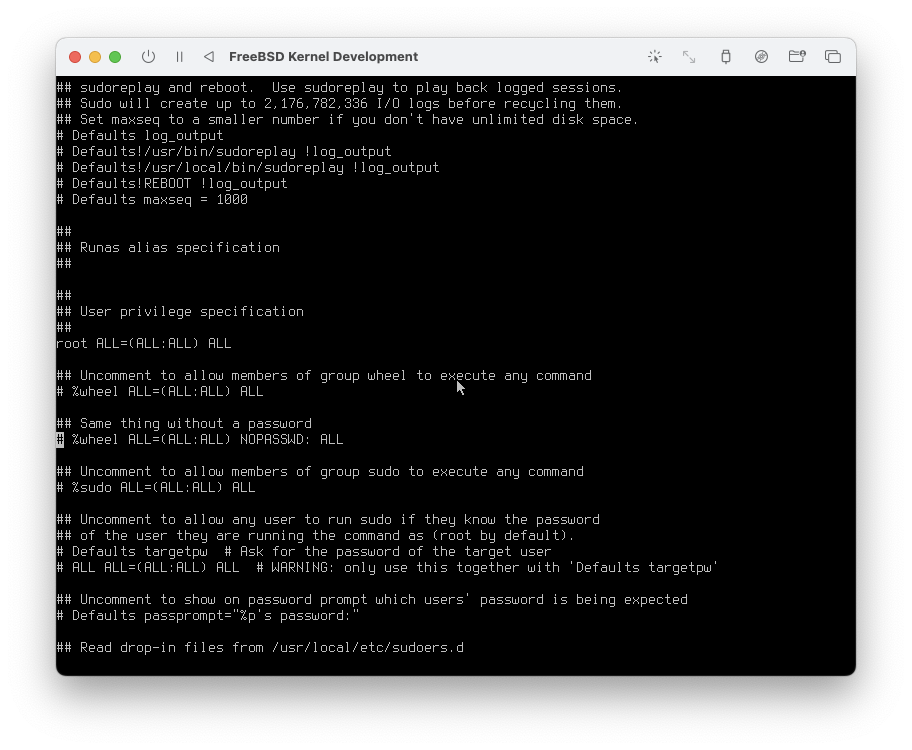
\includegraphics[width=0.6\linewidth]{46}
  \caption{Go to the line to uncomment where wheel users can use sudo
    without a password.}
  \label{fig:utm-fbsd-wheel}
\end{figure}

\begin{figure}
  \centering
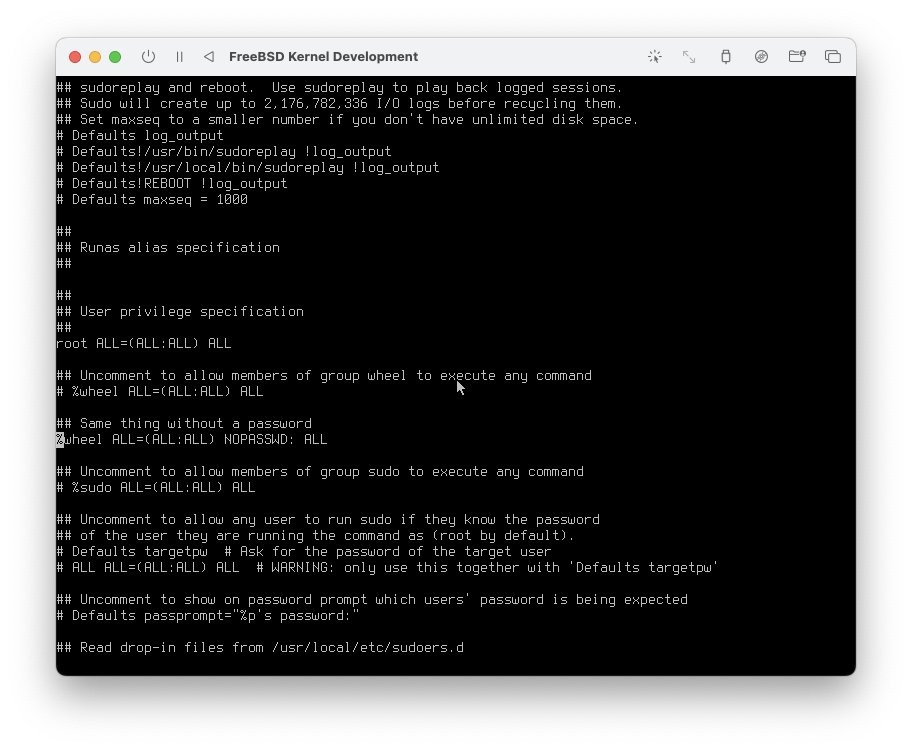
\includegraphics[width=0.6\linewidth]{47}
  \caption{Remove the comment (\#) character}
  \label{fig:umt-fbsd-uncomment}
\end{figure}

\begin{figure}
  \centering
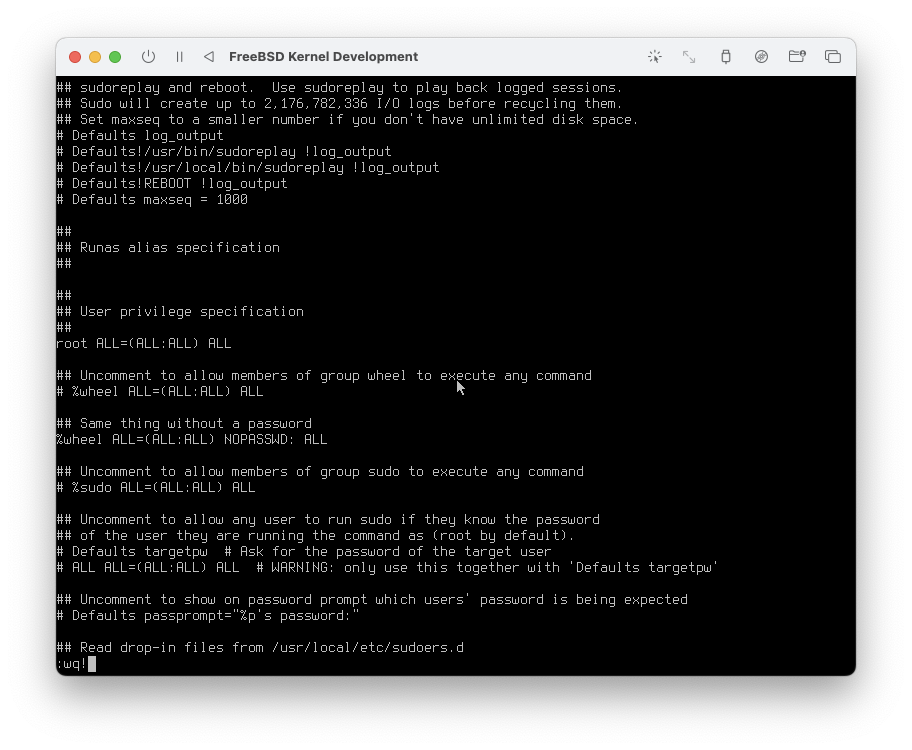
\includegraphics[width=0.6\linewidth]{49}
  \caption{Save and quit vi with the :wq! command sequence}
  \label{fig:utm-fbsd-wq}
\end{figure}

\begin{figure}
  \centering
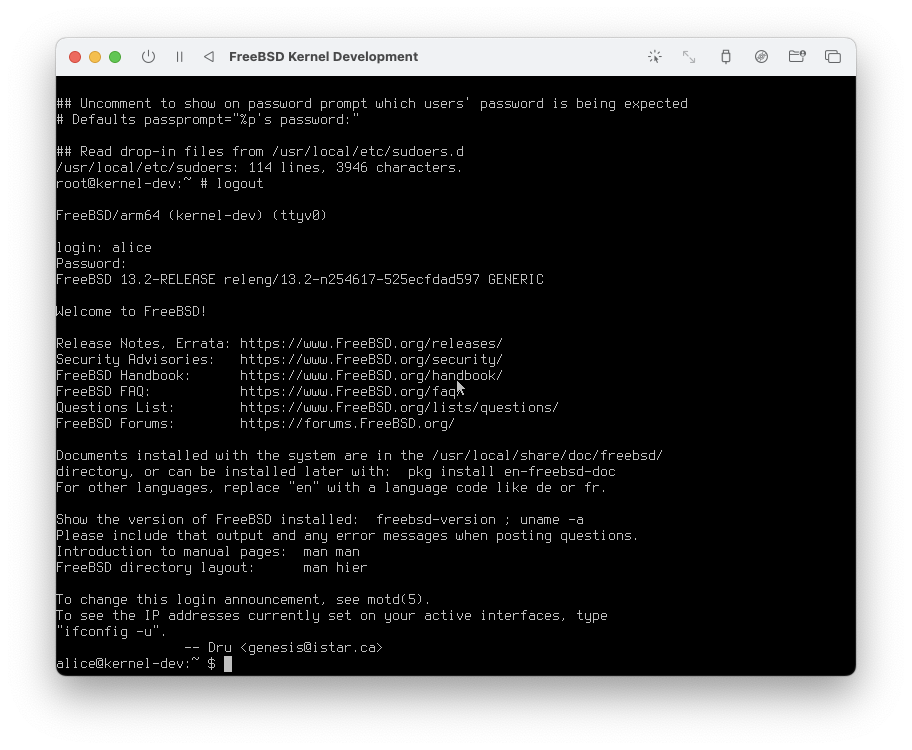
\includegraphics[width=0.6\linewidth]{50}
  \caption{Log into the system as a normal user}
  \label{fig:utm-fbsd-alice-login}
\end{figure}

\begin{figure}
  \centering
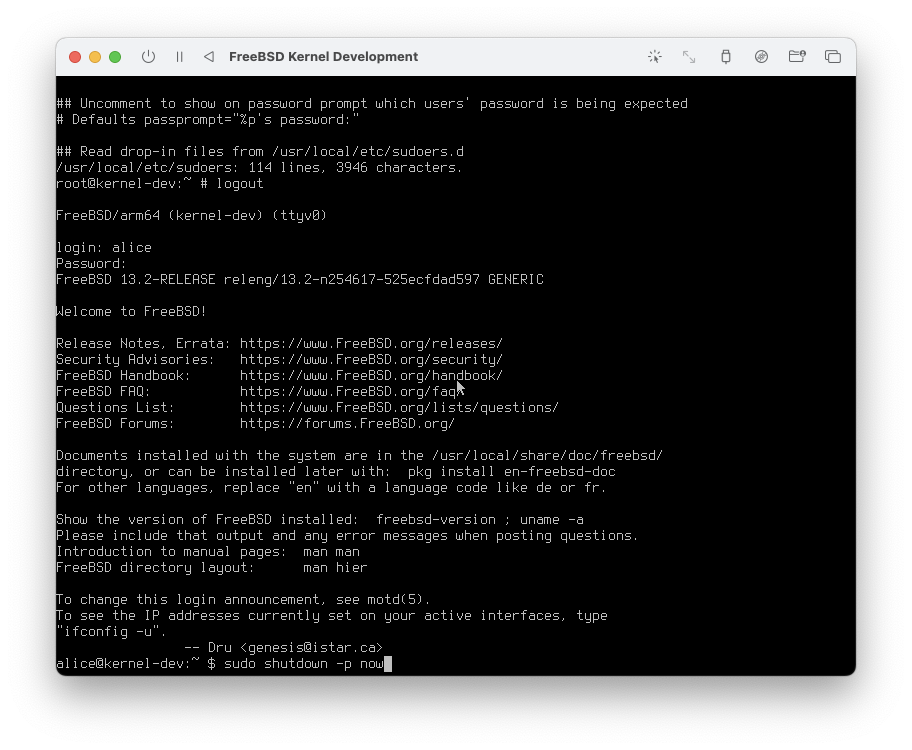
\includegraphics[width=0.6\linewidth]{51}
  \caption{Issue a shutdown with sudo as a normal user}
  \label{fig:utm-fbsd-shutdown}
\end{figure}

\begin{figure}
  \centering
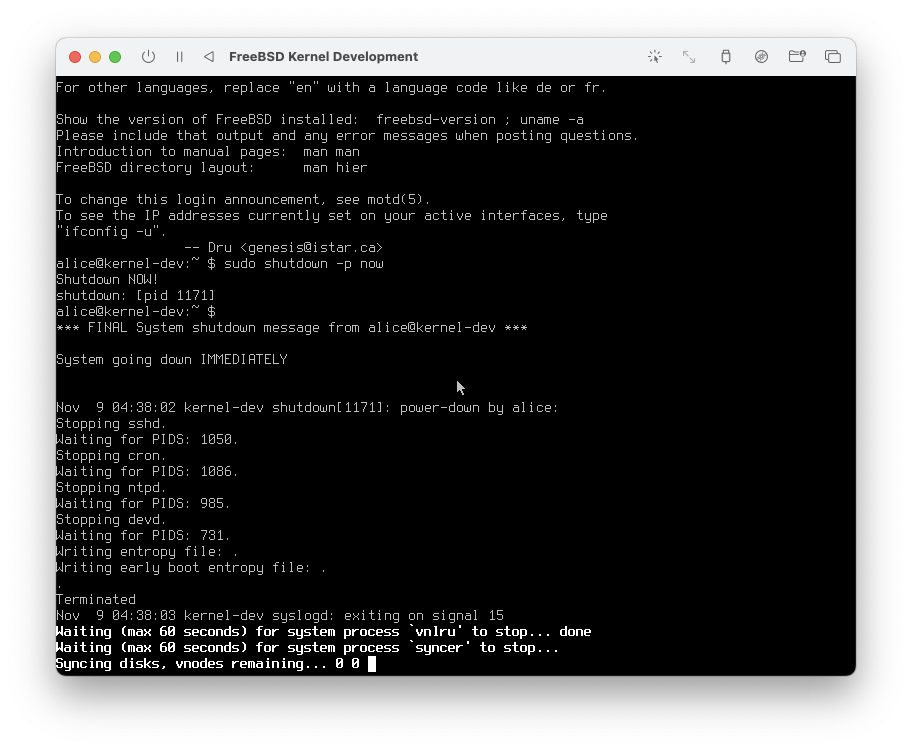
\includegraphics[width=0.6\linewidth]{52}
  \caption{System starts shutting down}
  \label{fig:utm-fbsd-shutdown-start}
\end{figure}

\begin{figure}
  \centering
\includegraphics[width=0.6\linewidth]{53}
  \caption{System shutdown complete, VM powers off}
  \label{fig:utm-fbsd-shutdown-done}
\end{figure}

\subsection{Creating a case sensitive volume.}
\label{sec:case-sensitive}

Most Unix-like operating systems are built on case sensitive
filesystems.  The filesystems on macOS are case preserving but not
case sensitive by default and this will be a problem if you try to
clone the FreeBSD source repository onto the default volume.  With the
Disk Utility you can create a case sensitive volume to store your
repositories.

\begin{figure}
  \centering
\includegraphics[width=0.6\linewidth]{54}
  \caption{Open Disk Utility and Select the Macintosh Volume}
  \label{fig:utm-mac-diskutil}
\end{figure}

\begin{figure}
  \centering
\includegraphics[width=0.6\linewidth]{55}
  \caption{Add a new, case sensitive, volume}
  \label{fig:utm-mac-case}
\end{figure}

\begin{figure}
  \centering
\includegraphics[width=0.6\linewidth]{56}
  \caption{Give the volume a useful name}
  \label{fig:utm-mac-name}
\end{figure}

Once you have your code cloned into the new volume you can mount the
volume over NFS into the FreeBSD VM.  You will need to log into the
virtual machine to see which IPv4 address it has been assigned.  In
Figure~\ref{fig:utm-fbsd-checkip} we see that our VM has an IP address
of 192.168.68.2, which means that the macOS host is 192.168.68.1, note
this down for later.

\begin{figure}
  \centering
\begin{verbatim}
ifconfig
vtnet0: flags=1008843<UP,BROADCAST,RUNNING,SIMPLEX,MULTICAST,LOWER_UP> metric 0 mtu 1500
	options=80028<VLAN_MTU,JUMBO_MTU,LINKSTATE>
	ether f6:d6:33:68:f7:0d
	inet 192.168.68.2 netmask 0xffffff00 broadcast 192.168.68.255
	media: Ethernet autoselect (10Gbase-T <full-duplex>)
	status: active
	nd6 options=29<PERFORMNUD,IFDISABLED,AUTO_LINKLOCAL>
lo0: flags=1008049<UP,LOOPBACK,RUNNING,MULTICAST,LOWER_UP> metric 0 mtu 16384
	options=680003<RXCSUM,TXCSUM,LINKSTATE,RXCSUM_IPV6,TXCSUM_IPV6>
	inet 127.0.0.1 netmask 0xff000000
	inet6 ::1 prefixlen 128
	inet6 fe80::1%lo0 prefixlen 64 scopeid 0x2
	groups: lo
	nd6 options=21<PERFORMNUD,AUTO_LINKLOCAL>
\end{verbatim}
  \caption{Check the virtual machine's IP address}
  \label{fig:utm-fbsd-checkip}
\end{figure}

On the macOS host we set up a file called \verb|/etc/exports| as shown
in Figure~\ref{fig:utm-mac-exports}

\begin{figure}
  \centering
\begin{verbatim}
cat /etc/exports
/Volumes/Repos -alldirs -maproot=0:0
\end{verbatim}
  \caption{Setting up the exports}
  \label{fig:utm-mac-exports}
\end{figure}

We next make sure the NFS daemon is running on the mac host.

\begin{figure}
  \centering
\begin{verbatim}
> sudo nfsd start
> sudo nfsd status
Password:
nfsd service is enabled
nfsd is running (pid 704, 8 threads)
\end{verbatim}
  \caption{Start NFS daemon}
  \label{fig:utm-mac-nfsd}
\end{figure}

Finally we mount the Repos volume into the virtual machine.

\begin{figure}
  \centering
\begin{verbatim}
> sudo mount -v -t nfs 192.168.68.1:/Volumes/Repos/Yale/freebsd-src /usr/src
> df /usr/src
Filesystem                                    1K-blocks       Used      Avail Capacity  Mounted on
192.168.68.1:/Volumes/Repos/Yale/freebsd-src 3902665360 2305897348 1596768012    59%    /usr/src
> ls /usr/src
ls /usr/src
CONTRIBUTING.md		bin			sbin
COPYRIGHT		cddl			secure
LOCKS			contrib			share
MAINTAINERS		crypto			stand
Makefile		etc			sys
Makefile.inc1		gnu			targets
Makefile.libcompat	include			tests
Makefile.sys.inc	kerberos5		tools
ObsoleteFiles.inc	lib			usr.bin
README.md		libexec			usr.sbin
RELNOTES		release
UPDATING		rescue
\end{verbatim}
  \caption{Mount the source volume}
  \label{fig:utm-fbsd-mount}
\end{figure}

You can now build a new kernel.

\begin{figure}
  \centering
\begin{verbatim}
> cd /usr/src
> sudo make -j 8 buildworld >& /tmp/bw.out

Check the output log in /tmp.bw.out

> sudo make -j 8 buildkernel >& /tmp/bk.out

Check the kernel build log in /tmp/bk.out
\end{verbatim}
  \caption{Build the world and the kernel}
  \label{fig:utm-fbsd-build}
\end{figure}

\end{document}


